\chapter{Results and Analysis\label{cha:results_analysis}}

The results chapter deals with presenting the different metrics discussed so far, within the RECAT-EU scheme. The data subset for the analysis was limited to four pair categories from the ICAO scheme: H-H, H-M, M-H and M-M. This simplification was done in order to filter out the small number of data points for other pairs, insufficient for any valid estimations of the distribution of inter-arrival distance or the landing time intervals. 

The distribution of inter-arrival distances for the RECAT-EU pairs were examined in agreement with the RECAT-EU reference separations. The arrival runway occupancy time (AROT) and the landing time interval (LTI) for particular pairs were compared to identify the limiting factor for throughput capacity. The AROT was considered limiting for the runway capacity if its frequency distribution overlapped excessively with the frequency distribution of the LTI. As mentioned earlier in the introduction section, no aircraft landing is allowed if another aircraft is present on a designated runway. An overlap of AROT and LTI can indicate a landing incursion and lead to missed approach. 

\section{Aircraft Traffic Mix\label{sec:traffic_mix}}

The aircraft traffic mix is one of the components that affect runway capacity as mentioned in the Introduction section~\ref{sec:runway_capacity}. Analysing of the traffic mix outlines the main aircraft categories that will be considered for analysis, the portion of arrivals that will experience reduced wake turbulence separation minima along with estimate of the inter arrival distance characteristic of each pair. A simplified overview of the re-categorisation mechanism for BIKF is shown in Table~\ref{tab:wtc2recat_division}.

\begin{table}[h]
\centering
\resizebox{0.6\textwidth}{!}{%
\begin{tabular}{clcllc}
\multicolumn{3}{c}{\cellcolor[HTML]{34CDF9}HEAVY} &  &  & \cellcolor[HTML]{FD6864}LIGHT \\ \hline
\multicolumn{1}{|c|}{\cellcolor[HTML]{34CDF9}CAT-A} & \multicolumn{1}{c|}{\cellcolor[HTML]{34CDF9}CAT-B} & \multicolumn{1}{c|}{\cellcolor[HTML]{32CB00}CAT-C} & \multicolumn{1}{c|}{\cellcolor[HTML]{F8FF00}CAT-D} & \multicolumn{1}{c|}{\cellcolor[HTML]{F8FF00}CAT-E} & \multicolumn{1}{c|}{\cellcolor[HTML]{FFC702}CAT-F} \\ \hline
\multicolumn{1}{l}{} &  & \multicolumn{4}{c}{\cellcolor[HTML]{F8FF00}MEDIUM}
\end{tabular}%
}
\caption[Transition from ICAO WTC to RECAT-EU categories]{Transition from ICAO WTC to RECAT-EU categories. CAT-C combines aircraft from the ICAO Heavy and Medium categories and CAT-F combines aircraft from the Medium and Light categories. The categorisation process and criteria for assigning an existing aircraft type into RECAT-EU scheme is illustrated in detail in Figure~\ref{fig:RECAT_criteria}.}
\label{tab:wtc2recat_division}
\end{table}

Sorting the aircraft fleet arriving at BIKF into ICAO WTC reveals that the majority of flights~(85,4\%) are in the Medium wake category and the rest are mainly in the Heavy category~(14,2\%) with less than one percent Light aircraft~(Figure~\ref{fig:post_fast_exit_mix_pie_v2}). The small portion of Light flights can be explained with the policy of air traffic control at BIKF to avoid servicing those flights during the morning and afternoon peaks. This distribution of the three categories implies that combining the aircraft into arriving pairs would produce primarily Medium-Medium (M-M) pairs. This is confirmed later by the analysis of the number of arrival pairs in the ICAO categories (Table~\ref{tab:pairs_mix_to_wtc}).

\begin{figure}[h]
    \centering
    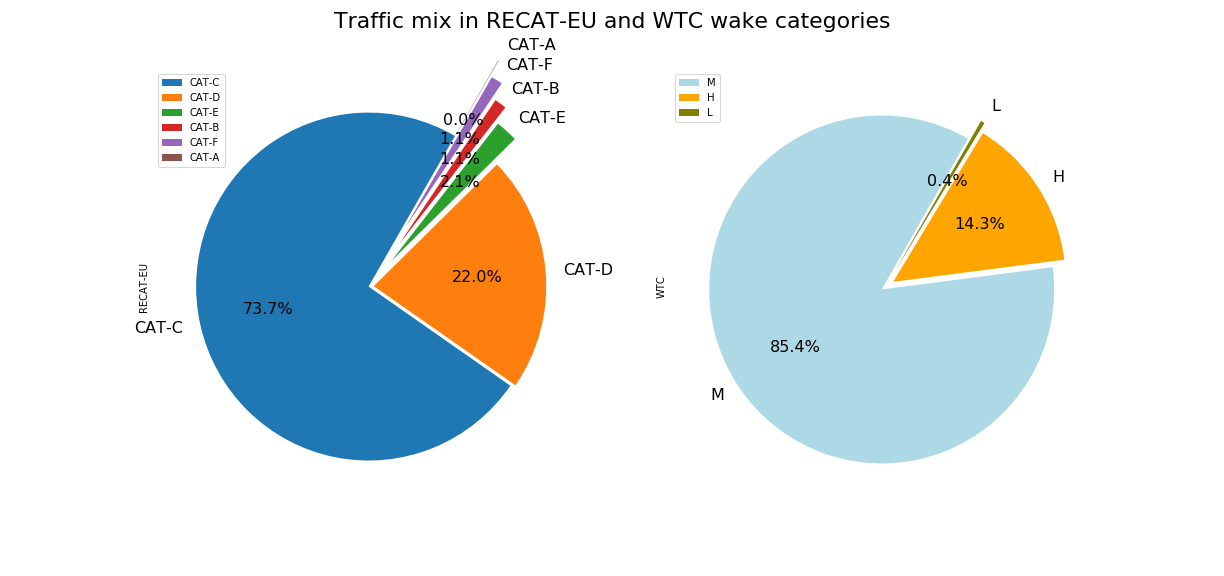
\includegraphics[width=1\textwidth]{graphics/fig_post_fast_exit_mix_pie_v2.png}
    \caption[Traffic mix in RECAT-EU and ICAO WTC]{The traffic mix at Keflavik Airport during peak hours, represented in RECAT-EU categories alongside ICAO WTC. The observed time period is 14 months starting October 2017.}
    \label{fig:post_fast_exit_mix_pie_v2}
\end{figure}

When this same fleet mix is presented using the RECAT-EU categories, the prevailing category is CAT-C (73,6\%), followed by CAT-D (22,1\%)~(Figure~\ref{fig:post_fast_exit_mix_pie_v2}). The percentage of each of the remaining categories varies but does not exceed 2\%. The expectation that this distribution of the RECAT-EU categories would result in primarily in C-C pairs is confirmed later on by the numbers presented in Table~\ref{tab:pairs_mix_to_recat}. 

Another approach for classification of the traffic fleet mix at BIKF during peak hours was to identify the aircraft types or models. The traffic data contains ICAO aircraft type designator, which is a two-, three- or four-character code composed of numbers and letters. This designator is unique for each aircraft type. The top fifteen aircraft types of the aircraft mix with their ICAO and RECAT-EU categories are presented in Figure~\ref{fig:traffic_mix_by_model}. Dominating the scene (56,8\% of all arrivals during peak hours) is the Boeing~757-200 model (ICAO: B752), followed by the Boeing~767-300 (ICAO: B763).

\begin{figure}[h]
    \centering
    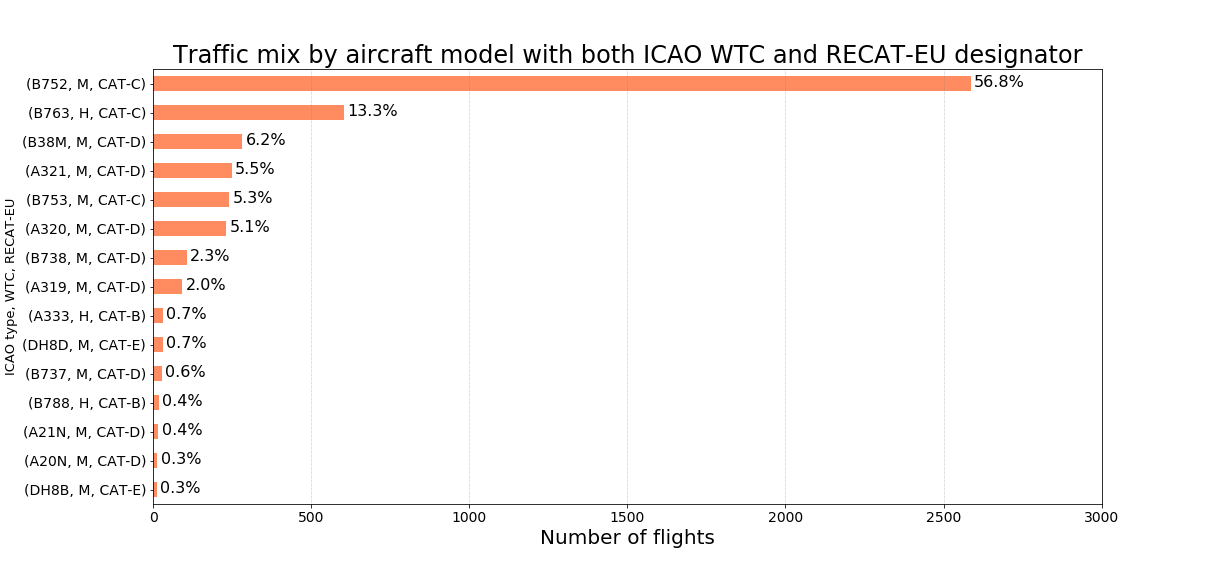
\includegraphics[width=1\textwidth]{graphics/fig_traffic_mix_by_model.png}
    \caption[Traffic mix by aircraft type.]{The traffic mix at Keflavik Airport during peak hours, grouped by aircraft type are shown alongside the ICAO WTC and RECAT-EU designators. The top three types comprise the major part of the Icelandair fleet. The observed time period is 14 months starting October 2017.}
    \label{fig:traffic_mix_by_model}
\end{figure}

 Those aircraft types represent a major part of the Icelandair fleet~\cite{icelandair_fleet} and the share of the Boeing~737~MAX~8 (ICAO: B38M) is likely to increase as the Icelandair company plans to gradually add sixteen new B38M and B39M models from the beginning of 2018. Flights arriving during peak hours for the observed period and operated by Icelandair are 76.2\% with 6,3\% of those being B38M flights. The tendency is towards increasing the share of the Medium WTC (or the CAT-D RECAT-EU category respectively), with the addition of the new aircraft to the Icelandair fleet.

\section{Arrival Runway Occupancy Time Considerations}\label{sec:AROT_considerations} 

\subsection{Traffic Mix and AROT\label{ssec:mix_effect_arot}}

Several approaches were used to look at the AROT at the airfield. First the runway occupancy was inspected based on the RECAT-EU category of the arrival aircraft in peak hours (Figure~\ref{fig:RECAT_AROTs_boxplot}).

\begin{figure}[h]
    \centering
    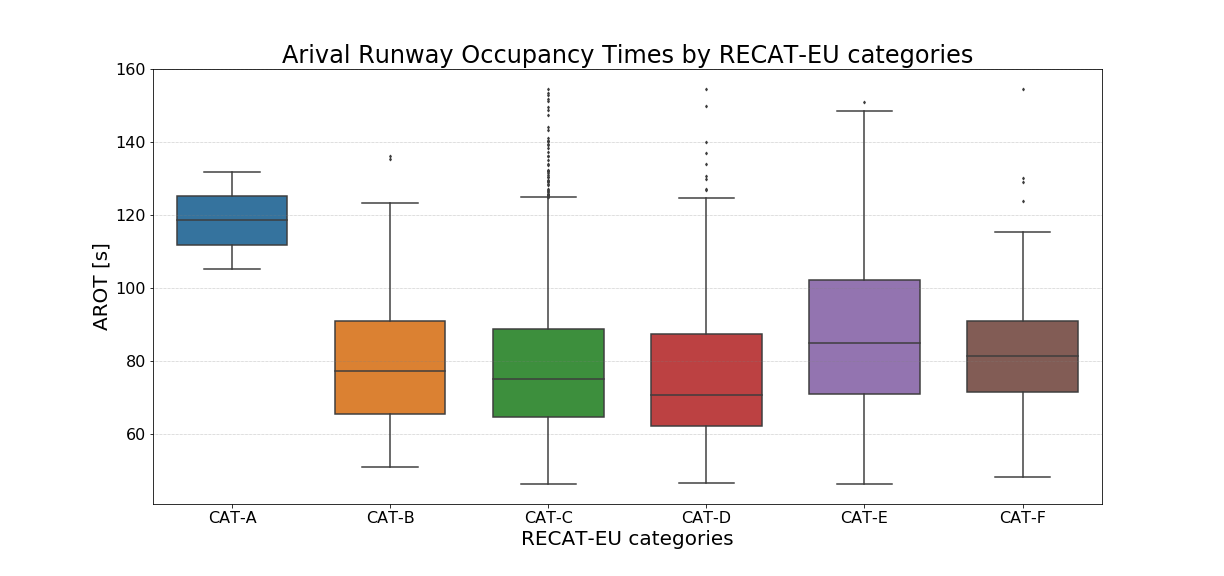
\includegraphics[width=1\textwidth]{graphics/fig_RECAT_AROTs_boxplot.png}
    \caption[AROTs box-plot for RECAT-EU categories, all runways]{Arrival Runway Occupancy Times for the different RECAT-EU categories based on data gathered for a period 14 months since October 2017. The coloured blocks indicate where 50\% of the data are located, or the inter-quartile range (IQR); lower edge is the 25\textsuperscript{th}~percentile (Q1), upper edge is the 75\textsuperscript{th}~percentile (Q3). The whiskers are at Q1-1,5$\times$IQR and Q3+1,5$\times$IQR.  The box plot shows the AROTs for all runways at BIKF during peak hours.}
    \label{fig:RECAT_AROTs_boxplot}
\end{figure}

The analysis showed that the shortest AROTs relate to aircraft from the CAT-D and CAT-C with mean values of 75 and 78 seconds respectively, as seen from the statistical analysis in (Table~\ref{tab:AROT_RECAT_stats}). These are also the two main categories that are considered in this study.

\begin{table}[h]
\centering
\resizebox{0.8\textwidth}{!}{%
\begin{tabular}{lr|r|r|r|r|r|r|r|}
\cline{3-9}
                          & \multicolumn{1}{c|}{}   & \multicolumn{7}{c|}{AROT [s]} \\ \hline
\multicolumn{1}{|l|}{RECAT-EU} & count & mean & std & min & 25\% & 50\% & 75\% & max \\ \hline
\multicolumn{1}{|l|}{CAT-A}    & 2     & 119  & 19  & 105 & 112  & 119  & 125  & 132 \\ \hline
\multicolumn{1}{|l|}{CAT-B}    & 53    & 81   & 20  & 51  & 65   & 77   & 91   & 136 \\ \hline
\multicolumn{1}{|l|}{CAT-C}    & 3447  & 78   & 17  & 46  & 65   & 75   & 89   & 155 \\ \hline
\multicolumn{1}{|l|}{CAT-D}    & 1034  & 75   & 18  & 46  & 62   & 71   & 87   & 155 \\ \hline
\multicolumn{1}{|l|}{CAT-E}    & 98   & 89   & 25  & 46  & 71   & 85   & 102  & 151 \\ \hline
\multicolumn{1}{|l|}{CAT-F}    & 49    & 83   & 22  & 48  & 72   & 81   & 91   & 155 \\ \hline
\end{tabular}%
}
\caption[AROTs for the air traffic mix by RECAT]{AROT statistics for the air traffic mix at BIKF by RECAT-EU categories. The count is the number of landings during peak hours since October 2017}
\label{tab:AROT_RECAT_stats}
\end{table}

The numbers also reveal that half of the aircraft from the CAT-C and CAT-D categories have AROTs in the range 60 to 90 seconds approximately, which outlines to some extent the anticipated values for AROT for the airfield. 

AROT is a metric that is expected to have minimal value, within certain safety limits, for increased throughput of the runway. One of the requirements for reducing the radar separation minimum (MRS) from 3~NM to 2,5~NM is AROT $\leq50$ seconds. ICAO Doc 4444 PANS-AM~\cite{doc44444} dictates that MSR may be reduced if the AROT of landing succeeding aircraft, which are established on the same final approach track is proven, by means such as data collection and statistical analysis and/or theoretical models, not to exceed 50 seconds. None of the average AROT values fulfils the 50~seconds limit for reduced MRS. This constraint fixes the MRS reference value at 3 NM and also suggest that the runway occupancy will be a limiting factor for the cases in which MRS is applicable (Table~\ref{tab:RECAT-dist}). This limitation is also confirmed by the statistical analysis for each of the runways in the following sections.% \ref{sssec:seasonal_arot}, \ref{sssec:runway_usage_arot}. 

\subsection{Seasonal Variation of AROT\label{ssec:seasonal_arot}}
Another approach was to analyse the seasonal variations of the runway occupancy time. The differentiation between summer and winter months was based on AROT values for a period of one year (Table~\ref{tab:month2season_arot}). Months with average AROT~$\leq$80~seconds formed the summer season and the rest were selected as winter months. This separation criteria is purely subjective but succeeds in forming two seasons with equal number of months. On average the seasonal difference of runway occupancy times was only eight seconds as seen in Table~\ref{tab:summer_winter_arot}. Still the seasonal variation should be taken into consideration as it can affect the AROT significantly, especially in the winter months when adverse weather conditions may impair the runway surface by accumulated slush, snow or ice, thus diminishing braking action. Good braking action due to runway surface condition is also one of the requirements for reduced MRS as provided by the procedures for navigation services of Air Traffic Management~\cite{doc44444}.

\begin{table}[h]
\centering
\resizebox{0.8\textwidth}{!} & \multicolumn{1}{l|}{50\%} & \multicolumn{1}{l|}{75\%} & \multicolumn{1}{l|}{max} \\ \hline
\multicolumn{1}{|l|}{SUMMER} & \multicolumn{1}{r|}{3727} & 76  & 17 & 46 & 63  & 72 & 87  & 155 \\ \hline
\multicolumn{1}{|l|}{WINTER} & \multicolumn{1}{r|}{956}  & 84  & 20 & 47 & 69  & 84 & 96  & 153 \\ \hline
\end{tabular}%
}
\caption[AROTs for the air traffic mix by season]{AROT statistics for the air traffic mix at BIKF by season. The count is the number of landings during peak hours over a 13 month period starting October 2017.}
\label{tab:summer_winter_arot}
\end{table}

\subsection{Runway Usage and AROT\label{ssec:runway_usage_arot}}
Runway usage for each of the runways was also examined both with regard to seasonal variations and rapid-exit taxiway usage. The usage of the four runways during peak hours is shown in Figure~\ref{fig:runway_usage_peak}. 

\begin{figure}[h]
    \centering
    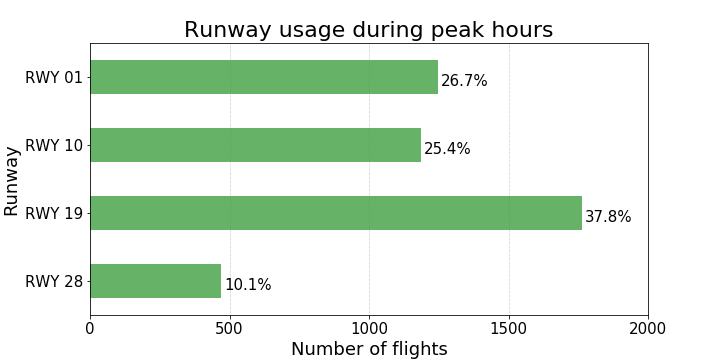
\includegraphics[width=0.8\textwidth]{graphics/fig_runway_usage_peak.png}
    \caption[Runway usage at BIKF during peak hours]{Runway usage at BIKF during peak hours for a period of 14 months starting October 2017. RWY-19 is the most frequently used runway, followed by RWY-01 and RWY-10. The RWY-01 is connected to rapid-exit TWY~A-1 and RWY-28 to rapid-exit TWY~B-1.}
    \label{fig:runway_usage_peak}
\end{figure}

BIKF airfield is currently equipped with two rapid-exit taxiways designated as TWY~A-1 and TWY~B-1. The first was completed on 26~July~2017 and the latter on 4~October~2017. Taxiway A-1 provides a rapid-exit track to the left for RWY-01, in the north landing direction, and B-1 serves RWY-28 exiting to the right in the west direction. The day that B-1 became operational was chosen as the starting time for the data set considered for analysis in this project. The reason behind this is the beneficial effect that rapid-exits have on reducing arrival runway occupancy time. 

The statistical analysis points to decreased AROT on average for RWY-01 with the use of A-1 (Table~\ref{tab:season_AROT_stats_RWY01_pre_fast_exit},~\ref{tab:season_AROT_stats_RWY01_post_fast_exit}). 

\begin{table}[h]
    \centering
    \subfloat[\label{tab:season_AROT_stats_RWY01_pre_fast_exit}]{\resizebox{0.8\textwidth}{!}{\begin{tabular}{lr|r|r|r|r|r|r|r|}
    \cline{3-9}
    \multicolumn{2}{l|}{RWY01}  & \multicolumn{7}{c|}{AROT {[}s{]}} \\ \hline
    \multicolumn{1}{|l|}{season} & count & \multicolumn{1}{l|}{mean} & \multicolumn{1}{l|}{std} & \multicolumn{1}{l|}{min} & \multicolumn{1}{l|}{25\%} & \multicolumn{1}{l|}{50\%} & \multicolumn{1}{l|}{75\%} & \multicolumn{1}{l|}{max} \\ \hline
    \multicolumn{1}{|l|}{Summer} & \multicolumn{1}{r|}{1346} & 94 & 15 & 48 & 84 & 93 & 103 & 152 \\ \hline
    \multicolumn{1}{|l|}{Winter} & \multicolumn{1}{r|}{192} & 103 & 19 & 50 & 90 & 100 & 115 & 153 \\ \hline
    \end{tabular}}}
    
    \subfloat[\label{tab:season_AROT_stats_RWY01_post_fast_exit}]{\resizebox{0.8\textwidth}{!}{\begin{tabular}{lr|r|r|r|r|r|r|r|}
\cline{3-9}
\multicolumn{2}{l|}{RWY01, TWY A-1}  & \multicolumn{7}{c|}{AROT  {[}s{]}} \\ \hline
\multicolumn{1}{|l|}{season} & count & \multicolumn{1}{l|}{mean} & \multicolumn{1}{l|}{std} & \multicolumn{1}{l|}{min} & \multicolumn{1}{l|}{25\%} & \multicolumn{1}{l|}{50\%} & \multicolumn{1}{l|}{75\%} & \multicolumn{1}{l|}{max} \\ \hline
\multicolumn{1}{|l|}{Summer} & \multicolumn{1}{r|}{533} & 57 & 8 & 46 & 52 & 56 & 60 & 130 \\ \hline
\multicolumn{1}{|l|}{Winter} & \multicolumn{1}{r|}{98} & 60 & 10 & 47 & 54 & 58 & 64 & 101 \\ \hline
\end{tabular}}}

\caption[AROTs RWY-01 with and without rapid-exit by season]{AROTs for runway RWY-01 by season: \protect\subref{tab:season_AROT_stats_RWY01_pre_fast_exit} without rapid-exit and \protect\subref{tab:season_AROT_stats_RWY01_post_fast_exit} with rapid-exit TWY A-1. The count is the number of landings during peak hours from July 2017 to November 2018.}

\end{table}

This decrease of AROT for flights using TWY~A-1, during the winter season was 42\% and 39\% for the summer months. Still, judging by the number of arrivals during peak hours, the rapid-exit is used by less than 1/3 of the flights. The comparatively lower usage of rapid-exit TWY~A-1, can be linked to its layout and the fact that A-1 exits into TWY~E-3, meeting taxiing aircraft in the opposite direction (Figure~\ref{fig:BIKF_schematic}), so the rapid-exit is avoided altogether during peak hours.

\begin{figure}[h]
    \centering
    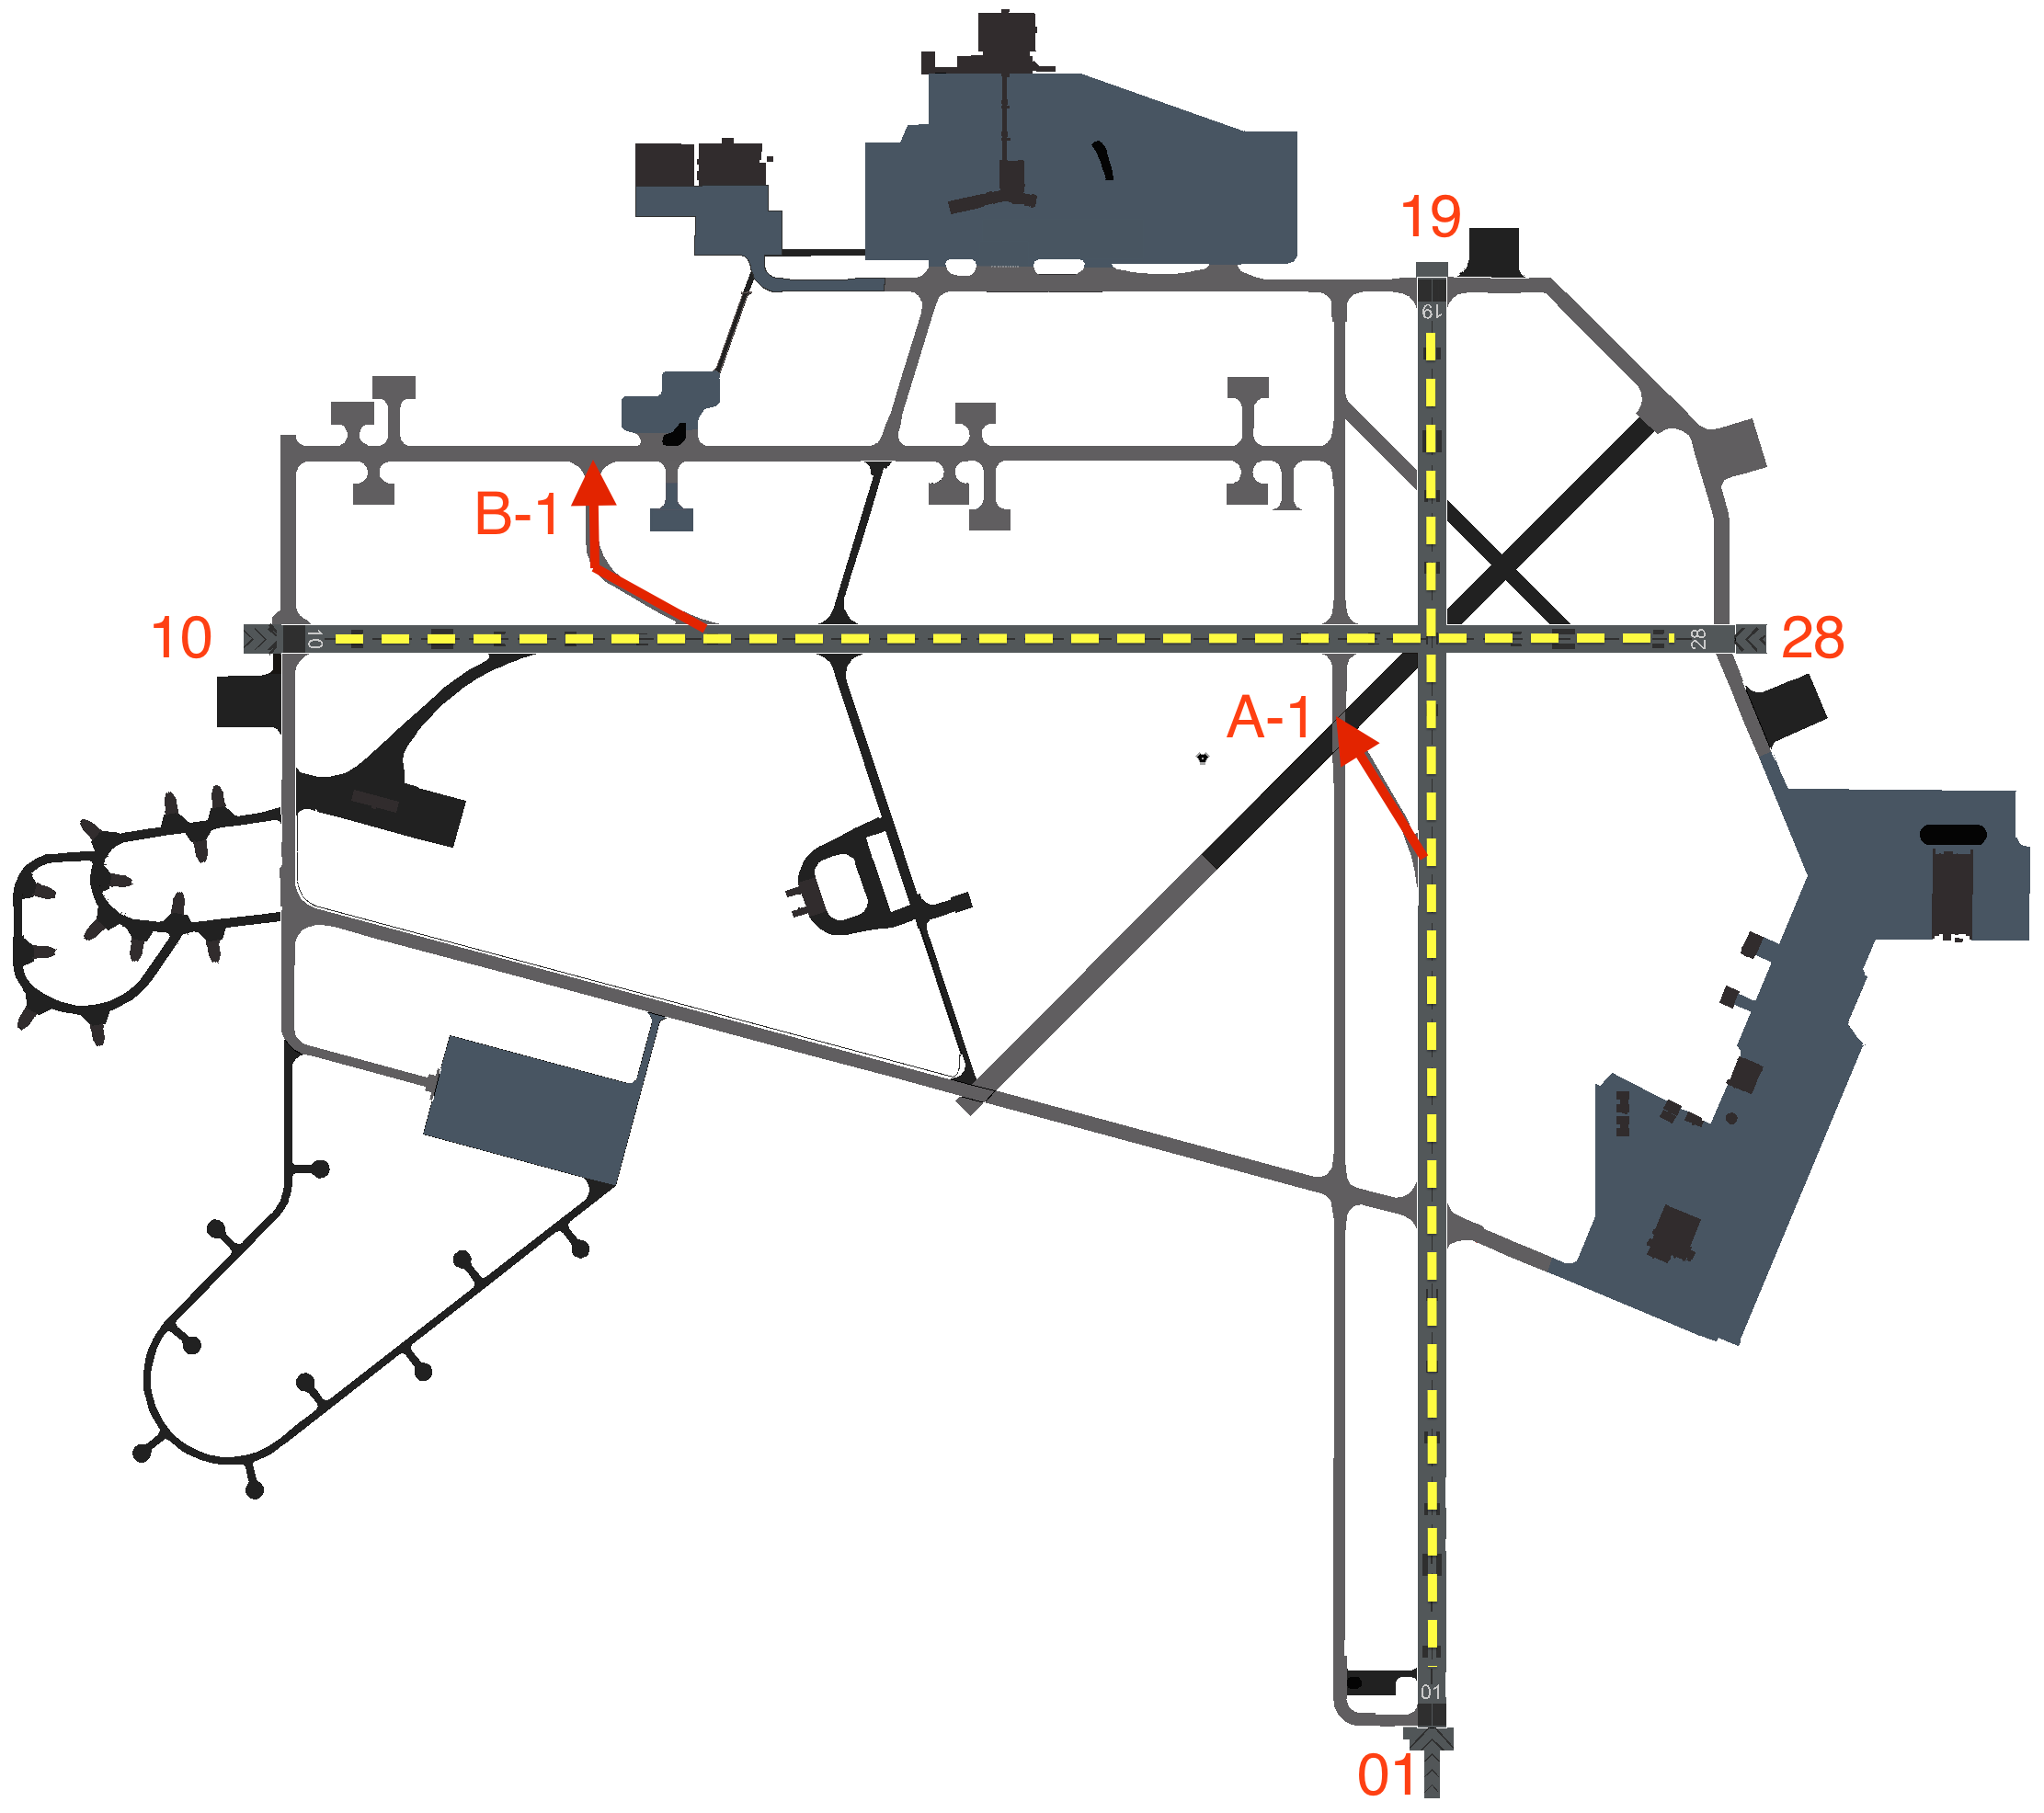
\includegraphics[width=1\textwidth]{graphics/BIKF_schematic.png}
    \caption[BIKF schematic]{BIKF schematic with four marked runways in perpendicular configuration (dashed yellow lines) and two rapid-exit taxiways (red arrows): TWY~A-1 on RWY~01 and TWY~B-1 on RWY~28 (source:~ Isavia).}
    \label{fig:BIKF_schematic}
\end{figure}

The data for RWY-28 present a somewhat different picture. After the implementation of TWY~B-1 in the end of 2017, arriving flights use almost exclusively the rapid-exit. The average AROT is being reduced by 33\% for the summer months and by 34\% for the winter, with the usage of rapid-exit taxiway (Table~\ref{tab:season_AROT_stats_RWY28_pre_fast_exit},~\ref{tab:season_AROT_stats_RWY28_post_fast_exit}). 

\begin{table}[h]
\centering
\resizebox{0.8\textwidth}{!} & \multicolumn{1}{l|}{50\%} & \multicolumn{1}{l|}{75\%} & \multicolumn{1}{l|}{max} \\ \hline
\multicolumn{1}{|l|}{Summer} & \multicolumn{1}{r|}{550} & 99 & 13 & 46 & 90 & 98 & 105 & 155 \\ \hline
\multicolumn{1}{|l|}{Winter} & \multicolumn{1}{r|}{250} & 110 & 13 & 60 & 100 & 108 & 117 & 155 \\ \hline
\end{tabular}%
}
\caption[AROTs RWY-28 without rapid-exit by season]{AROTs for runway RWY-28 without rapid-exit, by season. The count is the number of landings during peak hours from October 2015 to November 2018. The time frame was intentionally increased to include more data points, as the flights that are not exiting through TWY~B-1 are drastically reduced after the implementation of the rapid-exit. The distribution of AROT does not present significant differences within the longer time frame}
\label{tab:season_AROT_stats_RWY28_pre_fast_exit}
\end{table}

\begin{table}[h]
\centering
\resizebox{0.8\textwidth}{!} & \multicolumn{1}{l|}{50\%} & \multicolumn{1}{l|}{75\%} & \multicolumn{1}{l|}{max} \\ \hline
\multicolumn{1}{|l|}{Summer} & 376 & 66 & 8 & 49 & 60 & 65 & 70 & 92 \\ \hline
\multicolumn{1}{|l|}{Winter} & 67 & 73 & 12 & 49 & 63 & 71 & 79 & 100 \\ \hline
\end{tabular}%
}
\caption[AROTs RWY-28 with rapid-exit by season]{AROTs for runway RWY-28 with rapid-exit TWY~B-1 by season. The count is the number of landings during peak hours from October 2017 to November 2018.}
\label{tab:season_AROT_stats_RWY28_post_fast_exit}
\end{table}

Despite the reduced AROT, runway RWY~28 remains least used, servicing only 10$\%$ of landing aircraft (Figure~\ref{fig:runway_usage_peak}). One explanation for the small share of landings on RWY-28 is that flights on approach for landing westwards are generally uncommon for BIKF. 

The preferred runway is RWY~19, servicing 37,8$\%$ of the arrivals. The larger share of RWY~19 and RWY-01 over the other two runways could be explained with the direction of approaching traffic during peak hours and the frequent northerly winds (\ref{fig:BIKF_wind_rose}), facilitating landing and decreased AROT, especially for RWY-01. Landings and take-offs are typically conducted into the wind and runways are usually designed so that the effect of the cross-wind component is mitigated~\cite[p.~301]{de_neufville_airport_2013}~\cite{manual1991_doc9157}.

\begin{table}[h]
\centering
\resizebox{0.8\textwidth}{!} & \multicolumn{1}{l|}{50\%} & \multicolumn{1}{l|}{75\%} & \multicolumn{1}{l|}{max} \\ \hline
\multicolumn{1}{|l|}{RWY 01} & 1253 & 86 & 23 & 46 & 66 & 88 & 101 & 153 \\ \hline
\multicolumn{1}{|l|}{RWY 10} & 1190 & 87 & 12 & 61 & 79 & 86 & 93 & 155 \\ \hline
\multicolumn{1}{|l|}{RWY 19} & 1770 & 68 & 10 & 46 & 62 & 66 & 71 & 155 \\ \hline
\multicolumn{1}{|l|}{RWY 28} & 470 & 69 & 14 & 49 & 61 & 66 & 74 & 155 \\ \hline
\end{tabular}%
}
\caption[AROTs during peak hours by runway]{AROT statistics for the air traffic mix at BIKF by runway. The count is the number of landings during peak hours from October 2017 to November 2018.}
\label{tab:all_RWY_AROT_stats}
\end{table}

A statistical summary for all the runways is shown in Table~\ref{tab:all_RWY_AROT_stats} and visualised in Figure~\ref{fig:runway_AROTs_boxplot}. The average AROT for the BIKF airfield amounted to 78 seconds with average standard deviation about the mean of 18 seconds. Overall, half of the landing aircraft occupy the runways between 67 and 85 seconds on average. 

\begin{figure}[h]
    \centering
    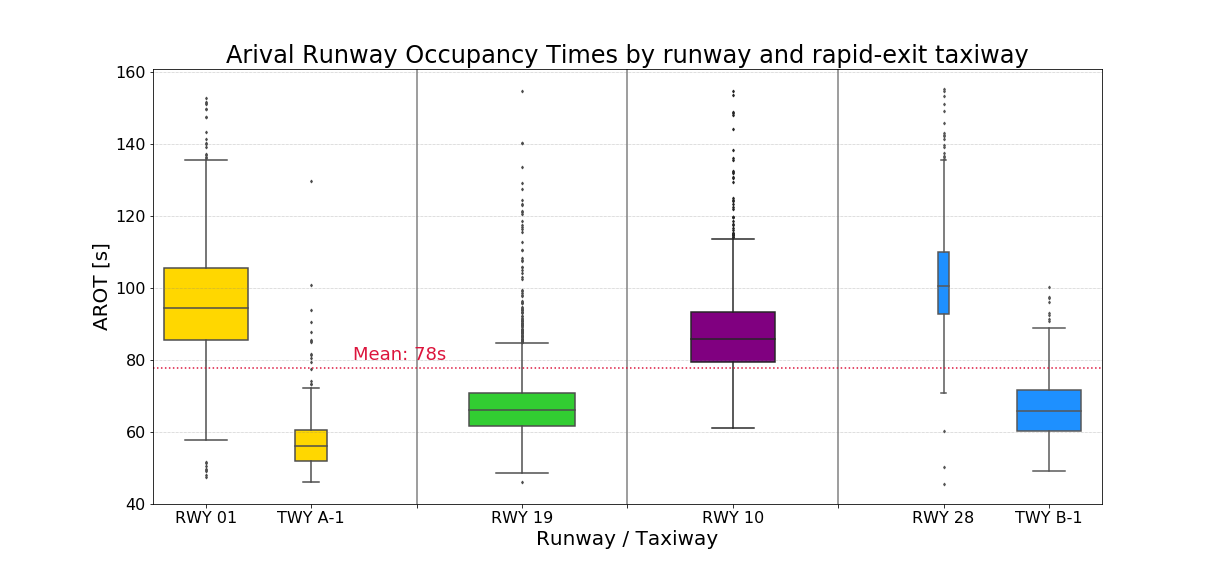
\includegraphics[width=1\textwidth]{graphics/fig_runway_AROTs_boxplot.png}
    \caption[AROTs box-plot per runway/taxiway]{Arrival Runway Occupancy Times at BIKF during peak hours for all runways with or without rapid-exit. The height coloured blocks indicate the inter-quartile range (IQR). The box-plots for RWY~01 and RWY~28 exclude arrivals using rapid-exit taxiways. TWY~A-1 and TWY~B-1 represent exclusively arrivals that use a runway's rapid-exit. The approximate share of arriving aircraft using a rapid-exit to those using the whole length of a runway is visualised by the width of the coloured blocks (not to scale). The average AROT value for BIKF is 78 seconds (dotted red line). The plot shows the AROTs based on data gathered for a period 14 months starting October 2017 with the exception of RWY~28 that includes arrivals since October 2015 (because of insufficient data points).}
    \label{fig:runway_AROTs_boxplot}
\end{figure}
% ---------------------------

\section{Inter-arrival Distance Separation}\label{sec:interarrival_dist_sep_RECAT}

The data set used for the analysis of the inter-arrival distances and the landing time interval combined information on landing aircraft from three data tables. A script in Isavia's internal GUI Vikingaskipið sorted the arrivals into a \textit{table of pairs} (leader and follower), with spacing and time interval between a leader and a follower calculated at the threshold. That table was merged with the \textit{key reference table}~(\ref{tab:sample_key_RECAT}) from EUROCONTROL to assign a RECAT-EU category to the leader and the follower. The \textit{data table of arrivals}~(\ref{tab:sample_df}) at BIKF added information about flights such as runway, taxiway and season. The resulting data-frame (Table~\ref{tab:sample_pairs}) contained the necessary information to allow estimate of the distribution of inter-arrival distances and LTI, based on wake turbulence category, for arriving pairs during peak hours.

\begin{table}[h]
\centering
\resizebox{\textwidth}{!}{%
\begin{tabular}{lllllllllllll}
lead\_type & follow\_type & lead\_wtc & follow\_wtc & arrival\_dist & time\_diff & lead\_recat & follow\_recat & runway & taxiway & oper & year & season \\ \hline
B752 & DH8D & M & M & 7.374 & 198 & CAT-C & CAT-E & RWY 19 & TWY S-2 & ICE & 2017  & summer \\
B752 & B763 & M & H & 6.682 & 161 & CAT-C & CAT-C & RWY 19 & TWY S-2 & ICE & 2017  & summer \\
B763 & B763 & H & H & 9.568 & 237 & CAT-C & CAT-C & RWY 19 & TWY S-2 & ICE & 2017  & summer \\
B763 & B752 & H & M & 7.365 & 208 & CAT-C & CAT-C & RWY 28 & TWY B-1 & ICE & 2017  & winter \\
B752 & GLF4 & M & M & 5.086 & 132 & CAT-C & CAT-E & RWY 01 & TWY A-1 & ICE & 2017  & winter
\end{tabular}%
}
\caption[Data table sample for arrival pairs at BIKF during peak hours]{Data table sample (abridged) used in the analysis of inter-arrival distance and landing time interval for aircraft pairs arriving at BIKF during peak hours. The units of the LTI (time\_diff) are seconds, distance (arrival\_dist) is measured in nautical miles.}
\label{tab:sample_pairs}
\end{table}

The information for the arrival pairs was fitted into the ICAO WTC scheme in order to recognise the prevailing aircraft pair mix, which is a consequence of the aircraft fleet mix discussed previously in Section~\ref{sec:traffic_mix}. Clearly the majority of arrival pairs were classified as Medium-Medium (M-M), as shown in Table~\ref{tab:pairs_mix_to_wtc}. The other noticeable pairs were variations of the Heavy and the Medium categories i.e. H-H, H-M and M-H. Those four pair types formed the subset of data to be further analysed and re-categorised into the RECAT-EU scheme. The rest of the pairs containing Light aircraft were discarded as being insignificant because of their limited number. 

\begin{table}[h]
\centering
\resizebox{0.3\textwidth}{!}{%
\begin{tabular}{cc|r|r|r|}
\cline{3-5}
\multicolumn{1}{l}{} & \multicolumn{1}{l|}{} & \multicolumn{3}{c|}{Follower} \\ \cline{3-5} 
\multicolumn{1}{l}{} & \multicolumn{1}{l|}{} & \multicolumn{1}{c|}{H} & \multicolumn{1}{c|}{M} & \multicolumn{1}{c|}{L} \\ \hline
\multicolumn{1}{|c|}{} & H & \cellcolor[HTML]{FFCC67}55 & \cellcolor[HTML]{FE996B}332 & \cellcolor[HTML]{FFFFC7}2 \\ \cline{2-5} 
\multicolumn{1}{|c|}{} & M & \cellcolor[HTML]{FE996B}367 & \cellcolor[HTML]{FD6864}1799 & \cellcolor[HTML]{FFFFC7}7 \\ \cline{2-5} 
\multicolumn{1}{|c|}{\multirow{-3}{*}{\rotatebox[origin=c]{90}{Leader}}} & L & \cellcolor[HTML]{FFFFC7}3 & \cellcolor[HTML]{FFFFC7}9 & \cellcolor[HTML]{FFFFC7}1 \\ \hline
\end{tabular}%
}
\caption[BIKF traffic mix sorted into ICAO WTC]{Number of ICAO pairs from the traffic mix at BIKF during peak hours, arranged into the corresponding wake category. The majority of aircraft pairs comprise the M-M category (69,9\%), followed by M-H (14,3\%), H-M (12,9\%) and H-H (2,1\%) pairs. The observation period is from October 2017 to November 2018.}
\label{tab:pairs_mix_to_wtc}
\end{table}

The ICAO WTC scheme specifies a distance separation minima as prescribed in  Table~\ref{tab:ICAO_WTC}. The distributions of the distance separations from the selected four pair-types were examined and presented in Figure~\ref{fig:dist_separ_HH_HM_MH_MM_pairs} along with the ICAO reference separation minima. 

\begin{figure}[h]
    \centering
    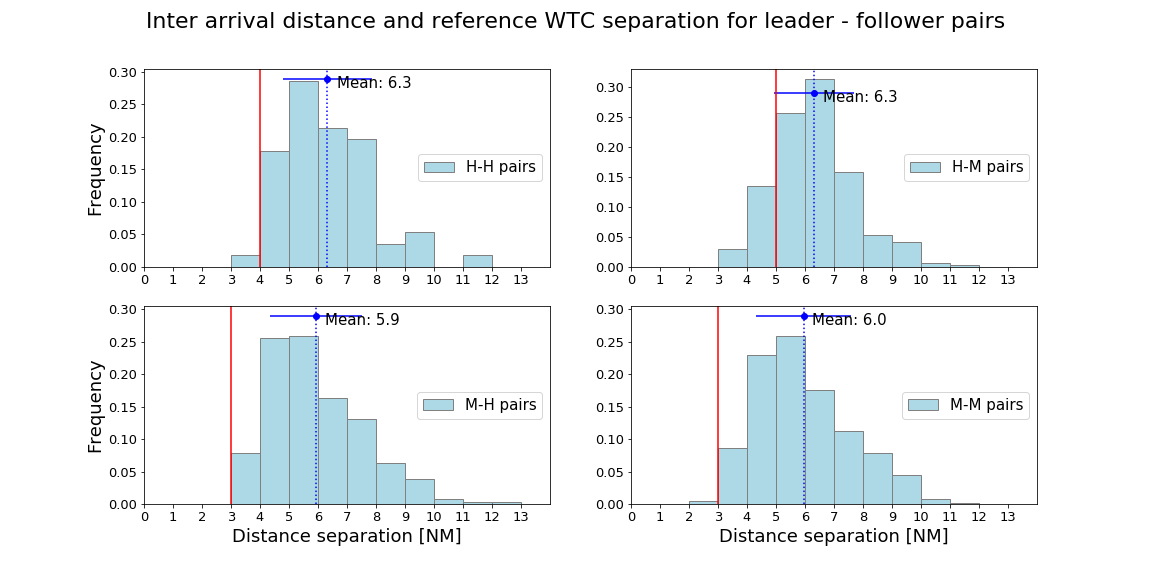
\includegraphics[width=1\textwidth]{graphics/fig_dist_separ_HH_HM_MH_MM_pairs.png}
    \caption[Inter-arrival distance separation, main ICAO pairs]{Distribution of the inter-arrival distance separation for selected ICAO pair categories. The red reference line indicates the separation minima for a particular pair category. The blue horizontal line indicates 1 standard deviation about the mean.}
    \label{fig:dist_separ_HH_HM_MH_MM_pairs}
\end{figure}

The portion of aircraft pairs that exhibit distance separation to the left of the ICAO reference minima can be attributed to flights operating under visual flight rules (VFR), according to Air Traffic Control (ATC) at BIKF. When visual flight rules are in effect, the separation may be decided by the pilot. Most of those flights are Icelandair operated aircraft of B736 and B752 type, which are classified as Heavy and Medium ICAO wake category respectively, but end up in the same CAT-C category under the  RECAT-EU scheme. Practice at Keflavík airport has shown that the distance separation for this particular pair can be reduced under VFR by allowing the follower closer, but over the final approach flight path of the leader, hence the reduced spacing within some H-M pairs.

Each of the ICAO aircraft pairs were re-categorised, based on the RECAT-EU scheme. The visual representation within figures was simplified and considers a reduced data-set, again by filtering out the pair categories with insufficient number of data points. The mix of arrival pairs from the peak hour traffic at BIKF after re-categorisation is presented in Table~\ref{tab:pairs_mix_to_recat}. As expected from the traffic fleet analysis in Section~\ref{sec:traffic_mix}, most of the aircraft formed C-C pairs. The rest of the more significantly presented traffic pairs were combinations of CAT-C, CAT-D and CAT-E categories. 

\begin{table}[h]
\centering
\resizebox{0.8\textwidth}{!}{%
\begin{tabular}{cc|c|c|c|c|c|c|}
\cline{3-8}
\multicolumn{1}{l}{} & \multicolumn{1}{l|}{} & \multicolumn{6}{c|}{Follower} \\ \cline{3-8} 
\multicolumn{1}{l}{} & \multicolumn{1}{l|}{} & CAT-A & CAT-B & CAT-C & CAT-D & CAT-E & CAT-F \\ \hline
\multicolumn{1}{|c|}{} & CAT-A &  &  &  & \cellcolor[HTML]{FFFFC7}1 &  &  \\ \cline{2-8} 
\multicolumn{1}{|c|}{} & CAT-B &  & \cellcolor[HTML]{FFFFC7}1 & \cellcolor[HTML]{FFFC9E}17 & \cellcolor[HTML]{FFFC9E}16 & \cellcolor[HTML]{FFFFC7}2 &  \\ \cline{2-8} 
\multicolumn{1}{|c|}{} & CAT-C &  & \cellcolor[HTML]{FFFC9E}19 & \cellcolor[HTML]{FD6864}1689 & \cellcolor[HTML]{FE996B}241 & \cellcolor[HTML]{FFCE93}41 & \cellcolor[HTML]{FFFC9E}14 \\ \cline{2-8} 
\multicolumn{1}{|c|}{} & CAT-D & \cellcolor[HTML]{FFFFC7}1 & \cellcolor[HTML]{FFFC9E}10 & \cellcolor[HTML]{FE996B}229 & \cellcolor[HTML]{FE996B}199 & \cellcolor[HTML]{FFFC9E}12 & \cellcolor[HTML]{FFFFC7}5 \\ \cline{2-8} 
\multicolumn{1}{|c|}{} & CAT-E &  & \cellcolor[HTML]{FFFFC7}1 & \cellcolor[HTML]{FFCE93}42 & \cellcolor[HTML]{FFFFC7}10 &  &  \\ \cline{2-8} 
\multicolumn{1}{|c|}{\multirow{-6}{*}{\rotatebox[origin=c]{90}{Leader}}} & CAT-F &  &  & \cellcolor[HTML]{FFFC9E}16 & \cellcolor[HTML]{FFFFC7}8 & \cellcolor[HTML]{FFFFC7}1 &  \\ \hline
\end{tabular}}

\caption[BIKF traffic mix sorted into RECAT-EU categories]{Number of RECAT-EU pairs from the traffic mix at BIKF during peak hours, arranged into the corresponding wake categories. The majority of arrival pairs are classified as C-C (65,6\%) followed by C-D (9,4\%), D-C (8,9\%) and D-D (7,7\%) pairs. The observation period is from October 2017 to November 2018.}
\label{tab:pairs_mix_to_recat}
\end{table}

The RECAT-EU C-C pairs were formed primarily by ICAO Medium-Medium pairs. The reference separation minima for those pair types, in both wake separation schemes, is specified as 3~NM. Considering this, the outcome of re-categorising the ICAO~M-M pairs shows no apparent advantage in terms of separation, for the newly formed RECAT-EU pairs, presented mainly by the C-C pair category(Figure~\ref{fig:MM_to_RECAT_pairs_dist_separ}). The RECAT-EU reference separation minima does not change its position after re-categorisation to allow for any shift of the separation distribution of aircraft pairs. Nearly 98\% of the ICAO~M-M pairs will experience no change of wake separation under the RECAT-EU scheme.

\begin{figure}[h]
    \centering
    \subfloat[]{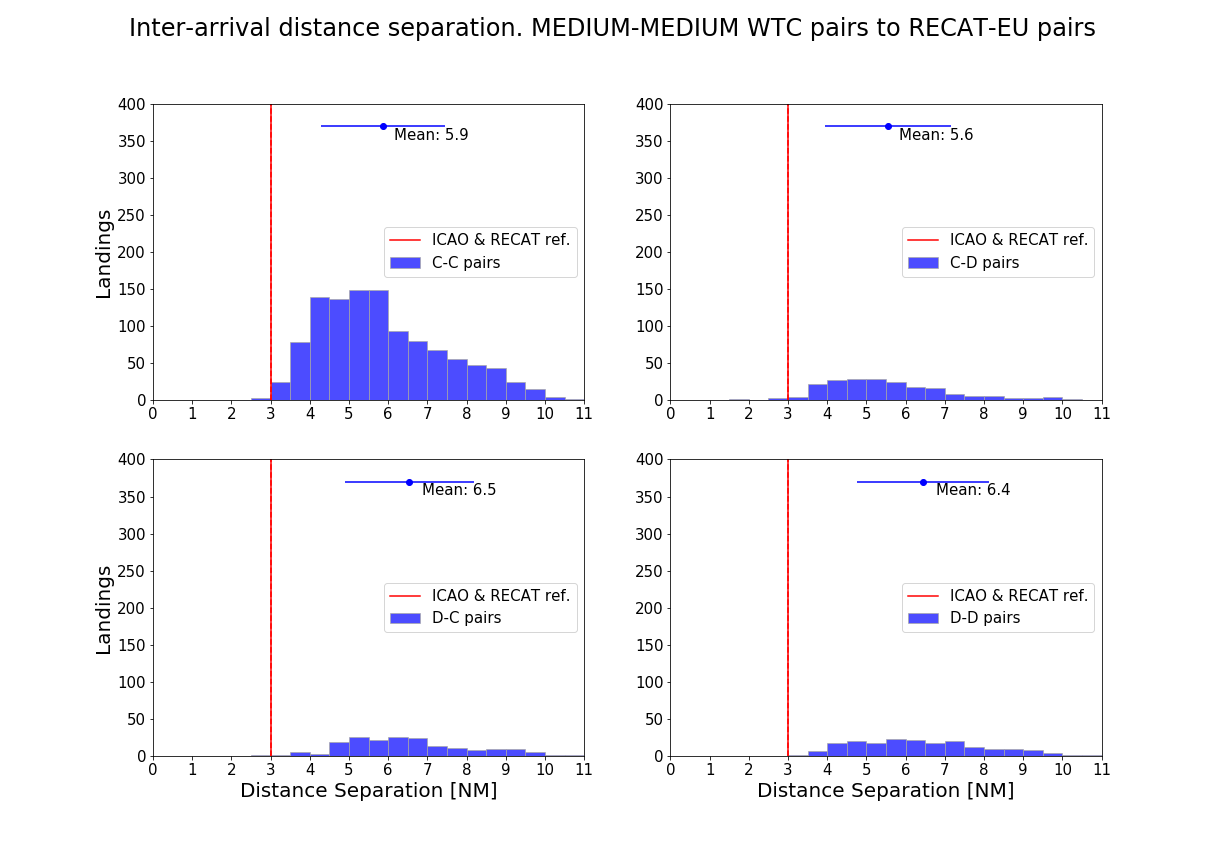
\includegraphics[width=1.0\textwidth]{graphics/fig_MM_to_RECAT_pairs_dist_separ.png}\label{mm2recat}}
    
    \vspace{1cm}
    
    \subfloat[]{\resizebox{0.5\textwidth}{!}{\begin{tabular}{|c|c|c|c|c|c|}
    \hline
    \multicolumn{2}{|c|}{} & \multicolumn{4}{c|}{Follower} \\ \cline{3-6} 
    \multicolumn{2}{|c|}{\multirow{-2}{*}{\begin{tabular}[c]{@{}c@{}}ICAO M-M pairs\\into RECAT-EU\end{tabular}}} & CAT-C & CAT-D & CAT-E & CAT-F \\ \hline
     & CAT-C & {\color[HTML]{3531FF} \textbf{1109}} & {\color[HTML]{3531FF} \textbf{205}} & \cellcolor[HTML]{FFCCC9}{\color[HTML]{3531FF} \textbf{29}} & \cellcolor[HTML]{FFCCC9}{\color[HTML]{3531FF} \textbf{9}} \\ \cline{2-6} 
     & CAT-D & {\color[HTML]{3531FF} \textbf{186}} & {\color[HTML]{3531FF} \textbf{194}} & 12 & \cellcolor[HTML]{FFCCC9}2 \\ \cline{2-6} 
     & CAT-E & 31 & 10 &  &  \\ \cline{2-6} 
    \multirow{-4}{*}{\rotatebox[origin=c]{90}{Leader}} & CAT-F & 7 & 5 &  &  \\ \hline
    \end{tabular}\label{number_mm2recat}}}
    
    \caption[Inter-arrival distance separation of ICAO M-M pairs into the RECAT-EU scheme]{\protect\subref{mm2recat} Distribution of the inter-arrival distance separation after re-categorisation of ICAO M-M pairs into the RECAT-EU scheme. The vertical red line indicate the separation minima in both wake schemes ICAO and RECAT-EU.\\ \protect\subref{number_mm2recat} Number of RECAT-EU pairs from the traffic mix at BIKF during peak hours, arranged into the corresponding wake categories. Numbers in blue are used in the representation of the distributions in~\protect\subref{mm2recat} and in Figure~\ref{fig:MM_to_CE_and_CF_pairs_dist_separ}. Red background pairs will experience increase in wake separation requirement compared to the same pairs under the ICAO scheme.}
    \label{fig:MM_to_RECAT_pairs_dist_separ}
\end{figure}
\clearpage
It is illustrative to mention also that some of the pair categories would suffer an increase in the required distance separation under the RECAT-EU scheme. Such example from the traffic at Keflavík airport would be the C-E and C-F pairs originating from the ICAO~M-M category~(Figure~\ref{fig:MM_to_CE_and_CF_pairs_dist_separ}). The separation minima in the former case would be moved from 3 NM up to 4 NM and in the latter case the increase is double, from 3 NM to 6 NM. Those pairs were rare in the data set and insufficient to reach any accurate estimate about the distribution of the current distance separation. 

\begin{figure}[h]
    \centering
    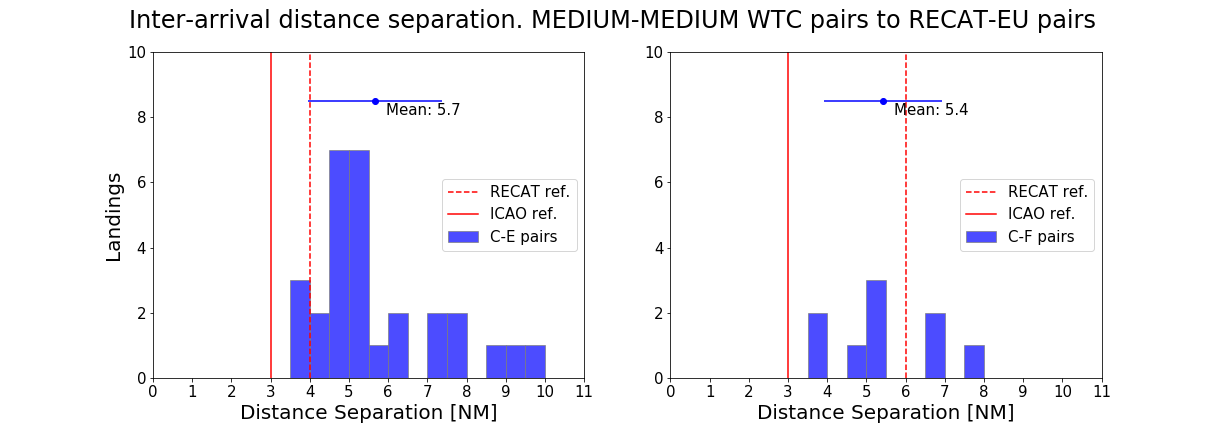
\includegraphics[width=1\textwidth]{graphics/fig_MM_to_CE_and_CF_pairs_dist_separ.png}
    \caption[Inter-arrival distance separation of ICAO M-M pairs into the RECAT-EU C-F and D-F pairs]{Distribution of the inter-arrival distance separation after re-categorisation of ICAO M-M pairs into the RECAT-EU C-E and C-F pairs. The vertical lines indicate the separation minima in different schemes (ICAO - solid red line, RECAT-EU - dashed red line).}
    \label{fig:MM_to_CE_and_CF_pairs_dist_separ}
\end{figure}
\clearpage
Similarly, the reference separation minima for all M-H pairs remains unchanged after re-categorisation~(Figure~\ref{fig:MH_to_RECAT_pairs_dist_separ}), which brings no decrease of separation under the RECAT-EU scheme for aircraft pairs originating from the ICAO~M-H category. 

\begin{figure}[h]
    \centering
    \subfloat[]{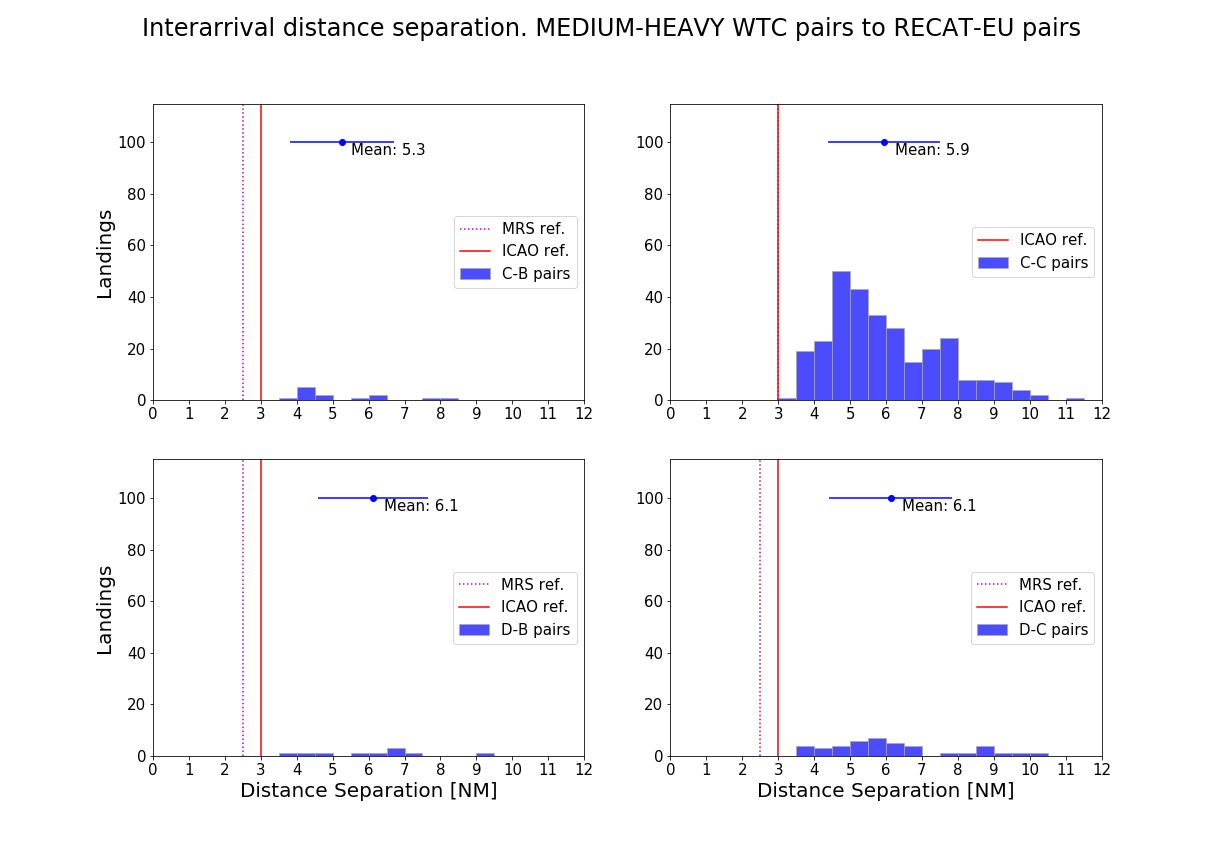
\includegraphics[width=1\textwidth]{graphics/fig_MH_to_RECAT_pairs_dist_separ.png}\label{mh2recat}}
    
    \vspace{1cm}
    
    \subfloat[]{\resizebox{0.5\textwidth}{!}{\begin{tabular}{|c|c|c|c|c|c|}
    \hline
    \multicolumn{2}{|c|}{} & \multicolumn{4}{c|}{Follower} \\ \cline{3-6} 
    \multicolumn{2}{|c|}{\multirow{-2}{*}{\begin{tabular}[c]{@{}c@{}}ICAO M-H pairs\\into RECAT-EU\end{tabular}}} & CAT-A & CAT-B & CAT-C & CAT-D \\ \hline
     & CAT-C &  & {\color[HTML]{3531FF} \textbf{13}} & {\color[HTML]{3531FF} \textbf{287}} &  \\ \cline{2-6} 
     & CAT-D & 1 & {\color[HTML]{3531FF} \textbf{10}} & {\color[HTML]{3531FF} \textbf{42}} & 2 \\ \cline{2-6} 
     & CAT-E & 1 & 9 &  &  \\ \cline{2-6} 
    \multirow{-4}{*}{\rotatebox[origin=c]{90}{Leader}} & CAT-F &  & 2 &  &  \\ \hline
    \end{tabular}\label{numbers_mh2recat}}}
    
    \caption[Inter-arrival distance separation of ICAO M-H pairs into the RECAT-EU scheme]{\protect\subref{mh2recat} Distribution of the inter-arrival distance separation after re-categorisation of ICAO M-H pairs into the RECAT-EU scheme. The vertical red line indicate the separation minima in both schemes ICAO and RECAT-EU.\\ \protect\subref{numbers_mh2recat} Number of RECAT-EU pairs from the traffic mix at BIKF during peak hours, arranged into the corresponding wake categories. Numbers in blue are used in the representation of the distributions in \protect\subref{mh2recat}.}
    \label{fig:MH_to_RECAT_pairs_dist_separ}
\end{figure}

For aircraft pairs of the ICAO H-M category, the transition to the RECAT-EU scheme results in reduced separation requirement. The reference separation minima for aircraft pairs that are re-categorised as B-C or B-D, shifts from 5 NM to 4 NM, while for the C-C and C-D pairs this reduction is 2~NM, from 5~NM to 3~NM (Figure~\ref{fig:HM_to_RECAT_pairs_dist_separ}). Approximately 99\% of the ICAO~H-M pairs will experience decrease of wake separation requirements under the RECAT-EU scheme.

\begin{figure}[h]
    \centering
    \subfloat[]{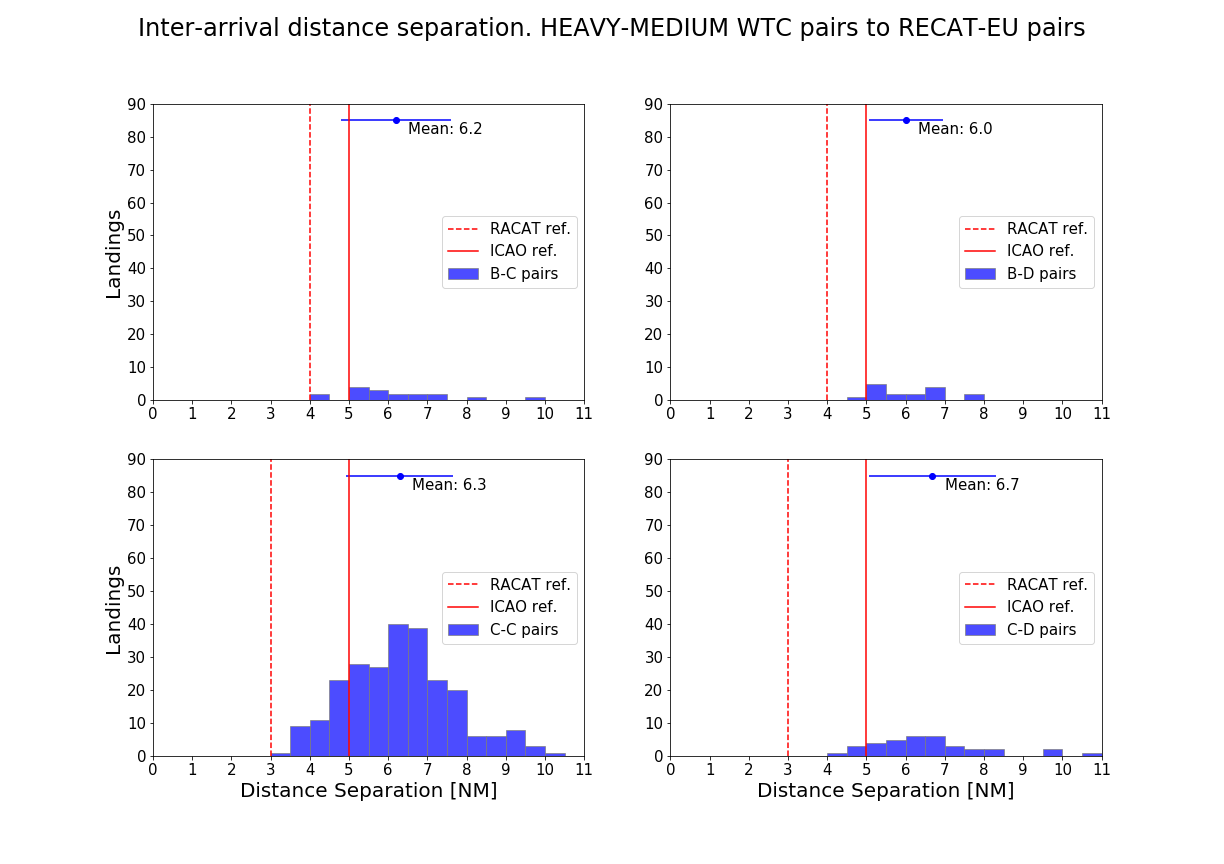
\includegraphics[width=1\textwidth]{graphics/fig_HM_to_RECAT_pairs_dist_separ.png}\label{hm2recat}}
    
    \vspace{1cm}
    
    \subfloat[]{\resizebox{0.5\textwidth}{!}{\begin{tabular}{|c|c|c|c|c|c|}
    \hline
    \multicolumn{2}{|c|}{} & \multicolumn{4}{c|}{Follower} \\ \cline{3-6} 
    \multicolumn{2}{|c|}{\multirow{-2}{*}{\begin{tabular}[c]{@{}c@{}}ICAO H-M pairs\\ into RECAT-EU\end{tabular}}} & CAT-C & CAT-D & CAT-E & CAT-F \\ \hline
     & CAT-A &  & 1 &  &  \\ \cline{2-6} 
     & CAT-B & \cellcolor[HTML]{9AFF99}{\color[HTML]{3531FF} \textbf{17}} & \cellcolor[HTML]{9AFF99}{\color[HTML]{3531FF} \textbf{16}} & 2 &  \\ \cline{2-6} 
     & CAT-C & \cellcolor[HTML]{9AFF99}{\color[HTML]{3531FF} \textbf{245}} & \cellcolor[HTML]{9AFF99}{\color[HTML]{3531FF} \textbf{36}} & \cellcolor[HTML]{9AFF99}10 & \cellcolor[HTML]{FFCCC9}1 \\ \cline{2-6} 
    \multirow{-4}{*}{\rotatebox[origin=c]{90}{Leader}} & CAT-D & \cellcolor[HTML]{9AFF99}1 & \cellcolor[HTML]{9AFF99}3 &  &  \\ \hline
    \end{tabular}\label{numbers_hm2recat}}}
    
    \caption[Inter-arrival distance separation of ICAO H-M pairs into the RECAT-EU scheme]{\protect\subref{hm2recat} Distribution of the inter-arrival distance separation after re-categorisation of ICAO H-M pairs into the RECAT-EU scheme. The vertical lines indicate the separation minima in different schemes (ICAO - solid red line, RECAT-EU - dashed red line).\\ \protect\subref{numbers_hm2recat} Number of RECAT-EU pairs from the traffic mix at BIKF during peak hours, arranged into the corresponding wake categories. Numbers in blue are used in the representation of the distributions in \protect\subref{hm2recat}. Green background pairs will experience reduced wake separation requirement under RECAT-EU and red background pairs will experience increase, compared to the same pairs under the ICAO scheme.}
    \label{fig:HM_to_RECAT_pairs_dist_separ}
\end{figure}

The ICAO H-H pairs were re-categorised primarily as C-C pairs into the RECAT-EU scheme (Figure~\ref{fig:HH_to_RECAT_pairs_dist_separ}). In this case, under RECAT-EU, the separation minima is reduced with one nautical mile (from 4 NM to 3 NM). All of the H-H pairs at BIKF during peak hours will experience this decreased separation requirement.

\begin{figure}[h]
    \centering
    \subfloat[]{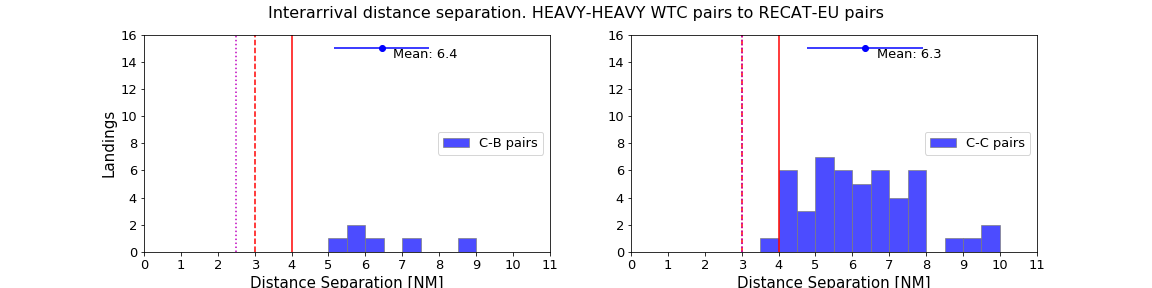
\includegraphics[width=1\textwidth]{graphics/fig_HH_to_RECAT_pairs_dist_separ.png}\label{hh2recat}}
    
    \vspace{1cm}
    
    \subfloat[]{\resizebox{0.35\textwidth}{!}{\begin{tabular}{|c|c|c|c|}
    \hline
    \multicolumn{2}{|c|}{} & \multicolumn{2}{c|}{Follower} \\ \cline{3-4} 
    \multicolumn{2}{|c|}{\multirow{-2}{*}{\begin{tabular}[c]{@{}c@{}}ICAO H-H pairs\\ into RECAT-EU\end{tabular}}} & CAT-B & CAT-C \\ \hline
     & CAT-B & \cellcolor[HTML]{9AFF99}1 &  \\ \cline{2-4} 
    \multirow{-2}{*}{Leader} & CAT-C & \cellcolor[HTML]{9AFF99}{\color[HTML]{3531FF} \textbf{6}} & \cellcolor[HTML]{9AFF99}{\color[HTML]{3531FF} \textbf{48}} \\ \hline
    \end{tabular}\label{numbers_hh2recat}}}
    
    \caption[Inter-arrival distance separation of ICAO H-H pairs into the RECAT-EU scheme]{\protect\subref{hh2recat} Distribution of the inter-arrival distance separation after re-categorisation of ICAO H-H pairs into the RECAT-EU scheme. The vertical lines indicate the separation minima in different schemes (ICAO - solid red line, RECAT-EU - dashed red line).\\ \protect\subref{numbers_hh2recat} Number of RECAT-EU pairs from the traffic mix at BIKF during peak hours, arranged into the corresponding wake categories. Numbers in blue are used in the representation of the distributions in \protect\subref{hh2recat}. Green background pairs will experience reduced wake separation requirement under RECAT-EU, compared to the same pairs under the ICAO scheme.}
    \label{fig:HH_to_RECAT_pairs_dist_separ}
\end{figure}

The share of the ICAO M-M pairs was the largest in the pair traffic mix at Keflaík International Airport. Most of those pairs end up in the C-C RECAT-EU category after re-categorisation and some experience change of the distance separation requirement. The share of aircraft pairs during peak hour traffic at BIKF, that will benefit from the re-categorisation, by reducing the required separation minima between aircraft is 14,9\%. An increase in separation requirement under RECAT-EU will suffer 1,6\% of the BIKF pairs. For the majority of pairs or 83,5\%, the re-categorisation will have no effect on the separation minima requirement between aircraft. 

The figures of the separation distribution and the separation minima are also evidence that incorporating the RECAT-EU scheme for the selected data-set, would potentially assist the aircraft pairs with a Heavy leader, but would not change much the situation for pairs with a Medium leader, in terms of separation requirement. In order to estimate the potential time savings from implementing the RECAT-EU scheme for Keflavík airport, the distance separation has to be transferred into the time domain, which is done by introducing the final approach speed in the following Section \ref{sec:LTI}.

\section{Landing Time Interval}\label{sec:LTI}

Another important metric derived from the data, together with the distance separation between pairs, was the landing time interval (LTI) that indicates whether AROT or the separation requirement is the limiting factor for airfield capacity. As mentioned in the study objective~(Section~\ref{sec:arot_and_study_objective}) the LTI quantifies the time separation between landing aircraft in a pair, calculated from the required distance separation and the final approach speed of the following aircraft. The final approach speed value for each arriving aircraft is in the \textit{bikf\_traffic} data table in the Isavia \textit{airport\_traffic} database. Isavia uses a script to calculate the final approach speed based on the ground speed measurement at 4 NM away from the runway threshold. 

The final approach speed used in calculating the reference time was set equal to the \textit{maximum average final approach speed} of landing aircraft from all four runways. This is done by finding the average speed for each of four runways and using the maximum of the four values as the final approach speed for each pair category. 

The reference time is analogous to the reference separation minima defined in the previous Section~\ref{sec:interarrival_dist_sep_RECAT}, i.e the reference time metric shifts its position under the RECAT-EU scheme. The aircraft considered for this calculation are exclusively from the Heavy and Medium wake categories, the ones dominating the traffic during peak hours at BIKF, so the final approach speed for those aircraft is approximately 146 knots in both cases (Table~\ref{tab:final_approach_max}).

\begin{table}[h]
\centering
\resizebox{.5\textwidth}{!}{%
\begin{tabular}{l|l|l|}
\cline{2-3}
 & \multicolumn{2}{l|}{Average final approach speed {[}knots{]}} \\ \cline{2-3} 
 & Heavy followers & Medium followers \\ \hline
\multicolumn{1}{|l|}{RWY 01} & 145,93 & \cellcolor[HTML]{FD6864}146,43 \\ \hline
\multicolumn{1}{|l|}{RWY 10} & 139,90 & 137,97 \\ \hline
\multicolumn{1}{|l|}{RWY 19} & 141,64 & 142,16 \\ \hline
\multicolumn{1}{|l|}{RWY 28} & \cellcolor[HTML]{FD6864}146,32 & 145,56 \\ \hline
\end{tabular}%
}
\caption[Maximum average final approach speeds]{Average final approach speeds for Heavy and Medium followers per runway. The final approach speed is calculated by Isavia from the aircraft ground speed at 4 nautical miles away from the threshold on approach for landing for each of the runways.}
\label{tab:final_approach_max}
\end{table}

Higher speed value results in lower reference time when the required separation minima per aircraft pair is considered. In this sense the reference time is a more liberally specified constraint, as opposed to using the minimum of the average approach speeds. This time was estimated for selected pairs (variations of the Heavy and the Medium categories, corresponding to the ones from Figure~\ref{fig:dist_separ_HH_HM_MH_MM_pairs}) and is presented in Figure~\ref{fig:time_separ_HH_HM_MH_MM_pairs} along with the LTI frequency distribution. Those pair categories represent the majority of the arrivals at BIKF during peak hours for a period of 14 month starting October 2017. The red time reference line indicates the time that a follower takes to travel the specified separation distance for the respective ICAO pair category.

\begin{figure}[h]
    \centering
    \subfloat[]{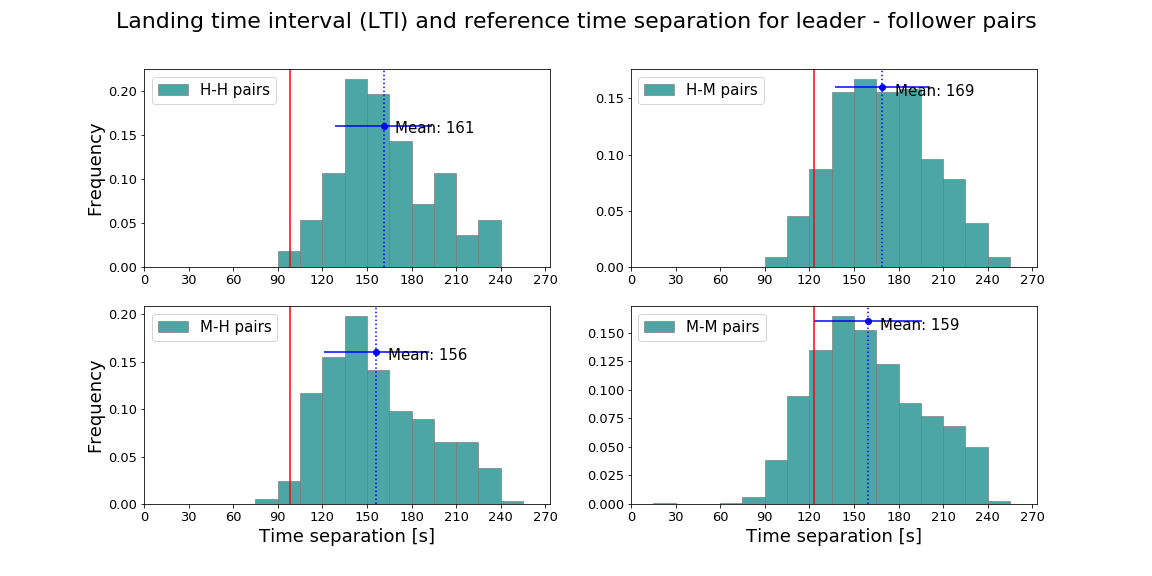
\includegraphics[width=1\textwidth]{graphics/fig_time_separ_HH_HM_MH_MM_pairs.png}\label{lti_distr}}
    
    \vspace{0.5cm}
    
    \subfloat[]{\resizebox{\textwidth}{!}{%
\begin{tabular}{cccc|c|c|c|c|c|c|c|c|}
\cline{5-12}
\multicolumn{4}{c|}{} & \multicolumn{4}{c|}{H follower} & \multicolumn{4}{c|}{M follower} \\ \cline{3-12} 
\multicolumn{2}{c|}{} & \multicolumn{2}{c|}{\begin{tabular}[c]{@{}c@{}}AROT\\  percentile range {[}s{]}\end{tabular}} &  & \multicolumn{2}{c|}{\begin{tabular}[c]{@{}c@{}}LTI \\ percentile range {[}s{]}\end{tabular}} &  &  & \multicolumn{2}{c|}{\begin{tabular}[c]{@{}c@{}}LTI \\ percentile range {[}s{]}\end{tabular}} &  \\ \cline{3-4} \cline{6-7} \cline{10-11}
\multicolumn{2}{c|}{\multirow{-2}{*}{}} & \multicolumn{1}{c|}{5\%} & 95\% & \multirow{-2}{*}{\begin{tabular}[c]{@{}c@{}}Reference \\ time {[}s{]}\end{tabular}} & 5\% & 95\% & \multirow{-2}{*}{Overlap {[}s{]}} & \multirow{-2}{*}{\begin{tabular}[c]{@{}c@{}}Reference\\ time {[}s{]}\end{tabular}} & 5\% & 95\% & \multirow{-2}{*}{Overlap {[}s{]}} \\ \hline
\multicolumn{1}{|c|}{} & \multicolumn{1}{c|}{H} & \multicolumn{1}{c|}{\cellcolor[HTML]{FFCE93}53} & \cellcolor[HTML]{FFCE93}\textbf{111} & {\color[HTML]{9A0000} 98} & \cellcolor[HTML]{68CBD0}\textbf{117} & \cellcolor[HTML]{68CBD0}215 & -- & {\color[HTML]{9A0000} 123} & \cellcolor[HTML]{68CBD0}\textbf{118} & \cellcolor[HTML]{68CBD0}224 & -- \\ \cline{2-12} 
\multicolumn{1}{|c|}{\multirow{-2}{*}{\rotatebox[origin=c]{90}{Leader}}} & \multicolumn{1}{c|}{M} & \multicolumn{1}{c|}{\cellcolor[HTML]{FFCE93}55} & \cellcolor[HTML]{FFCE93}\textbf{111} & {\color[HTML]{9A0000} 74} & \cellcolor[HTML]{68CBD0}\textbf{109} & \cellcolor[HTML]{68CBD0}220 & 2 & {\color[HTML]{9A0000} 74} & \cellcolor[HTML]{68CBD0}\textbf{105} & \cellcolor[HTML]{68CBD0}225 & 4 \\ \hline
\end{tabular}}\label{ref_times}}
    
\caption[Distribution of landing time interval (LTI) for ICAO pairs]{\protect\subref{lti_distr} Distribution of landing time intervals (LTI) for selected ICAO pair categories. The red line indicates a liberal time reference estimate for a particular pair category. The light blue field indicates the 5\%-95\% percentile range of landing time intervals. \\
\protect\subref{ref_times} Reference times calculated from the maximum final approach speed of the follower and the required separation minima per pair category, presented by the red vertical lines in \protect\subref{lti_distr}.}
\label{fig:time_separ_HH_HM_MH_MM_pairs}
\end{figure}

The shift from distance separation to time separation (between aircraft on approach for landing) is necessary in order to correlate the landing time interval (LTI) with the arrival runway occupancy time (AROT), both having the same dimension expressed in units of seconds.

Switching to the time domain can also provide an estimate of the potential time savings in the landing time intervals of arriving pairs, due to the RECAT-EU separation requirements. For the purpose, the change in the wake separation requirement, that some pairs experience, is divided by the maximum average final approach speed of the follower from a particular pair category. The change form ICAO to RECAT-EU in wake separation requirement can be up to 3 NM, as per Section~\ref{sec:interarrival_dist_sep_RECAT}. 

To illustrate the process of estimating the shift of reference times, let's consider the re-categorisation of ICAO Heavy-Medium pairs (Figure~\ref{fig:HM_to_RECAT_pairs_dist_separ}). The reduction of wake separation requirement for the resulting B-C, B-D and C-E pairs is 1 NM, while for the C-C, C-D, D-C and D-D pairs it is 2 NM. The maximum average final approach speed for a Medium follower from all runways at BIKF is 146,43 knots. This results in time difference of 25~seconds (-25,0\%) for decrease by 1 NM, or 49~seconds (-40,0\%) for decrease by 2 NM of the separation requirement. Here we also witness an increased separation requirement by 1 NM in the case of the C-E category, which will result in added 25 seconds (+33,3\%) to the reference time.

Lowered separation requirements reduce the time reference for some RECAT-EU landing pairs, but in other cases (C-F pairs originating from the ICAO M-M category, with increase in separation requirement by 3 NM) this reference time is increased by 100,0\%. Applying the method to the rest of the ICAO pair groups, that experience change in separation requirement, resulted in the time difference values shown in Table~\ref{tab:time_saving}.

\begin{table}[h]
\centering
\resizebox{.9\textwidth}{!}{%
\begin{tabular}{|c|c|c|c|c|c|c|c|}
\hline
\multicolumn{2}{|c|}{} & \multicolumn{6}{c|}{Follower} \\ \cline{3-8} 
\multicolumn{2}{|c|}{\multirow{-2}{*}{RECAT-EU scheme}} & CAT-A & CAT-B & CAT-C & CAT-D & CAT-E & CAT-F \\ \hline
 & CAT-A &  &  &  &  &  &  \\ \cline{2-8} 
 & CAT-B &  & \cellcolor[HTML]{9AFF99}-25s (-25\%) & \cellcolor[HTML]{9AFF99}-25s (-25\%) & \cellcolor[HTML]{9AFF99}-25s (-25\%) &  &  \\ \cline{2-8} 
 & CAT-C &  & \cellcolor[HTML]{9AFF99}-25s (-25\%) & \cellcolor[HTML]{9AFF99}-41s (-38\%) & \cellcolor[HTML]{9AFF99}-49s (-40\%) & \cellcolor[HTML]{ffccc9}+12s (+18\%) & \cellcolor[HTML]{ffccc9}+64s (+93\%) \\ \cline{2-8} 
 & CAT-D &  &  & \cellcolor[HTML]{9AFF99}-49s (-40\%) & \cellcolor[HTML]{9AFF99}-49s (-40\%) &  & \cellcolor[HTML]{ffccc9}+49s (+67\%) \\ \cline{2-8} 
 & CAT-E &  &  &  &  &  &  \\ \cline{2-8} 
\multirow{-6}{*}{\rotatebox[origin=c]{90}{Leader}} & CAT-F &  &  &  &  &  &  \\ \hline
\end{tabular}}
\caption[Reference time change for BIKF]{Reference time change between ICAO and RECAT-EU schemes. Green background pairs experience time savings and red background pairs suffer from increased reference time for landings. The values were averaged considering the number of aircraft pairs coming from the respective ICAO categories and the difference in separation requirements. The possible beneficial effect on landing time interval applies to 14,9\% of the pairs and for 1,6\% the LTI would have to increase. The re-categorisation will have no effect on the time reference for majority of the aircraft pairs (83,5\%), thus the lowered reference time is attributed primarily to ICAO pairs with a Heavy leader. The considered data is from arrivals during peak hours from October 2017 to November 2018.}
\label{tab:time_saving}
\end{table}

In view of the aircraft pairs that experience change in separation requirement under RECAT-EU, the time savings can potentially result in 35~seconds lower landing time interval on average or decreased LTI by 27,9\%. Those pair categories are indicated by a coloured background in Table~\ref{tab:time_saving} and comprise 14,9\% of the traffic during peak hours.

If the reference time shift is viewed in context of the overall traffic during peak hours at Keflavík Airport for the observed period the time savings correspond to 5,8 seconds on average per aircraft pair, or decreased LTI by 4,6\%. As mentioned before the re-categorisation will not influence the separation requirement for the majority of the aircraft pairs and for this decrease of the LTI contribute only the RECAT-EU pairs originating from ICAO Heavy leader pairs.


\fxnote{95\% Confidence intervals! and reference lines relation, assume safety relation between LTI distribution and reference minima}






\section{Constraints for Increased Capacity}% Runway Occupancy and Landing Time Interval for RECAT-EU pairs}

The following section presents the landing time intervals (LTI) for a subset of data points after re-categorisation from the ICAO wake turbulence scheme. The subset contained primarily C-C pairs. The C-C pairs were selected on the basis of being the more prominent subset with most of the data points. The LTI for the ICAO pair sets from \ref{sec:LTI} were modified to represent only the C-C pairs, where the effect on the LTI distribution after re-categorisation would be more accurate. The other metric used in contrast to the LTI was the arrival runway occupancy time for the respective aircraft pairs. The frequency distribution of the AROT included the runway occupancy for all the leaders of the selected ICAO category in order to make use of more data points and obtain a more general view on the AROT distribution. This decision was based on the assumption that the AROT of the leader in an aircraft pair is the constraint for the time separation of follower. This is illustrated in the result for the LTI and the AROT for the C-C pairs from H-H pair category in Figure~\ref{fig:CC_from_HH_pairs_time_sep}. 

\begin{figure}[h]
    \centering
    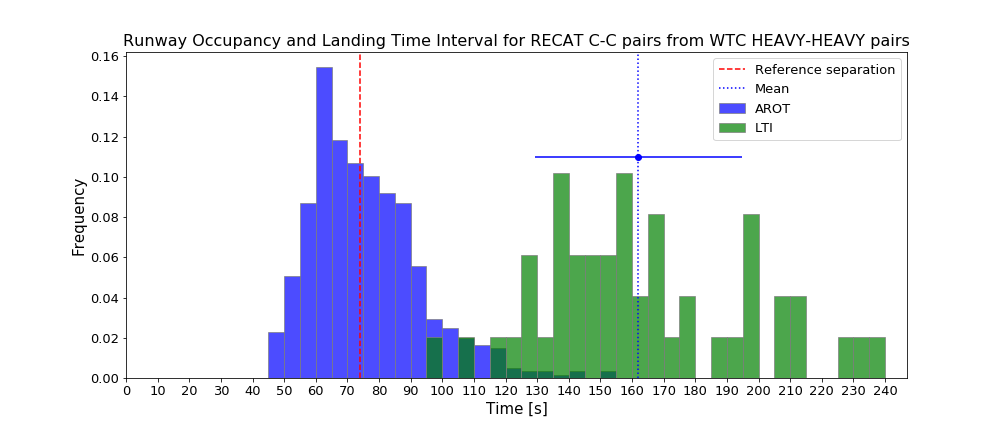
\includegraphics[width=1\textwidth]{graphics/fig_CC_from_HH_pairs_time_sep.png}
    \caption[AROT and LTI of C-C pairs originating from ICAO H-H pairs]{AROT and landing time intervals of C-C pairs originating from ICAO H-H pairs. The dashed red line indicates the RECAT-EU reference time separation for the C-C pairs. The blue horizontal line indicates 2 standard deviation left and right of the mean.}
    \label{fig:CC_from_HH_pairs_time_sep}
\end{figure}

The LTI frequency distribution contained all C-C pairs originating from the ICAO H-H category. The reference time separation (red dashed line) was calculated from the final approach speed and the RECAT-EU distance separation, as explained in \ref{sec:LTI}. The frequency distribution for the AROT, on the other hand, contained all pairs with CAT-C leader originating from the Heavy category, not only pairs with CAT-C leader and CAT-C follower. In this sense the distribution for the AROT was based on more data points than the distribution for the LTI and gave a more accurate presentation of the runway occupancy. Figure~\ref{fig:CC_from_HH_pairs_time_sep} represents the case for 1,9\% of all arrival pairs at BIKF for the observed period during peak hours.

The share of C-C pairs originating from the ICAO H-M category from the peak traffic at the airport was 9,5\%.  The LTI frequency distribution of those pairs is shown in Figure~\ref{fig:CC_from_HM_pairs_time_sep}. Here again the AROT distribution was based on the runway occupancy of CAT-C leaders, as in the previous case. 
 
\begin{figure}[h]
    \centering
    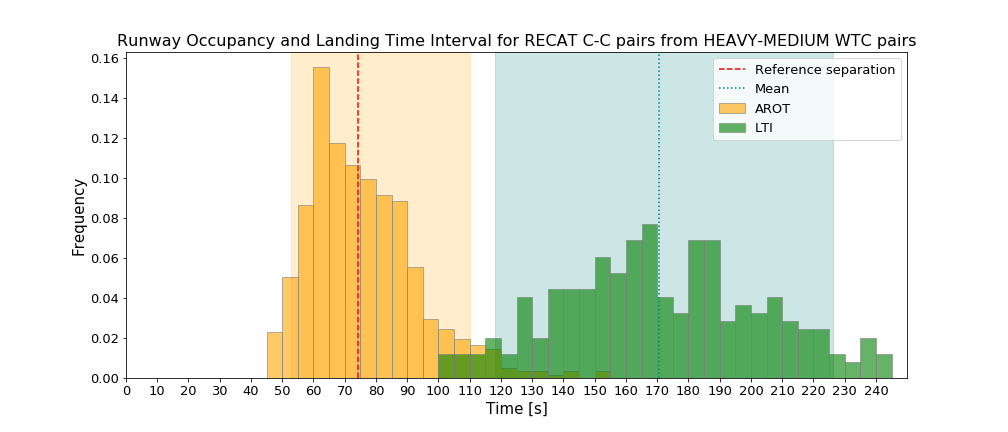
\includegraphics[width=1\textwidth]{graphics/fig_CC_from_HM_pairs_time_sep.png}
    \caption[AROT and LTI of C-C pairs originating from ICAO H-M pairs]{AROT and landing time intervals of C-C pairs originating from ICAO H-M pairs. The dashed red line indicates the RECAT-EU reference time separation for the C-C pairs. The blue horizontal line indicates 2 standard deviation left and right of the mean.}
    \label{fig:CC_from_HM_pairs_time_sep}
\end{figure}

These two cases: C-C pairs from ICAO H-H and H-M categories, would have more noticeable beneficial effect from the implementation of the RECAT-EU scheme (refer to~\ref{sec:interarrival_dist_sep_RECAT}). The decrease in distance separation in those cases is 1 NM or 2 NM. Translating the separation into the time domain resulted in a separation reference time line at 74 seconds and minimum LTI values close to 100 seconds. This shift of the reference line creates the potential for shift to the left in the frequency distribution of the LTI.
 
 \begin{figure}[h]
    \centering
    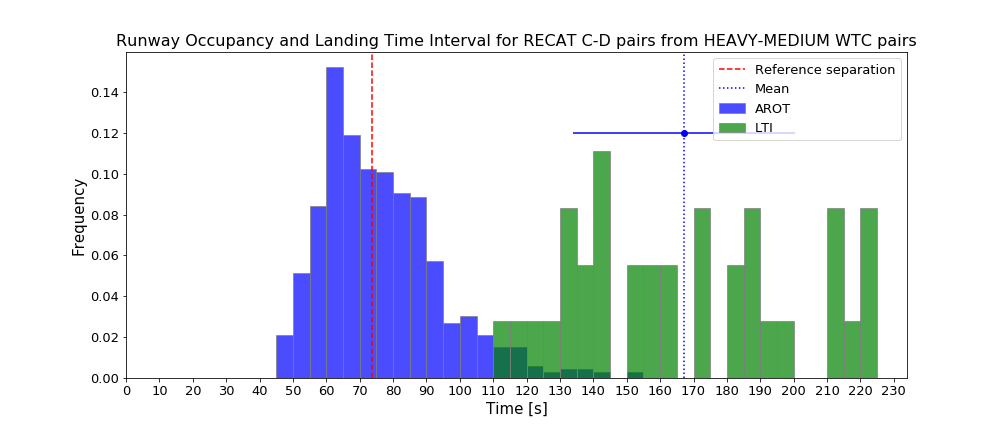
\includegraphics[width=1\textwidth]{graphics/fig_CD_from_HM_pairs_time_sep.png}
    \caption[AROT and LTI of C-D pairs originating from ICAO H-M pairs]{AROT and landing time intervals of C-D pairs originating from ICAO H-M pairs. The dashed red line indicates the RECAT-EU reference time separation for the C-D pairs. The blue horizontal line indicates 2 standard deviation left and right of the mean.}
    \label{fig:CD_from_HM_pairs_time_sep}
\end{figure}

Even greater potential for decrease of the inter-arrival time was observed in the case of C-D pairs from the ICAO H-M category (Figure~\ref{fig:CD_from_HM_pairs_time_sep}). Here the minimum LTI observed was 113 seconds, serving as a possible 39 seconds shift to the left of the frequency distribution. However the share of those pairs in the traffic was limited to 1.4\%.

The C-C pairs formed from the ICAO M-H category were 11,1\% from the BIKF traffic with frequency distribution of the LTI shown in Figure~\ref{fig:CC_from_MH_pairs_time_sep}. The reference line in this case is again at 74 seconds, and the LTI frequency distribution curve was closer to the reference than in the cases above.

\begin{figure}[h]
    \centering
    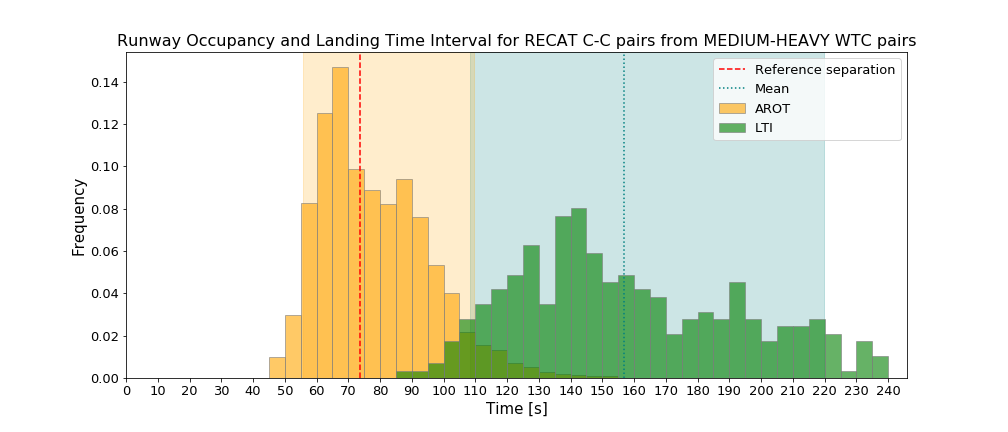
\includegraphics[width=1\textwidth]{graphics/fig_CC_from_MH_pairs_time_sep.png}
    \caption[AROT and LTI of C-C pairs originating from ICAO M-H pairs]{AROT and landing time intervals of C-C pairs originating from ICAO M-H pairs. The dashed red line indicates the RECAT-EU reference time separation for the C-C pairs. The blue horizontal line indicates 2 standard deviation left and right of the mean.}
    \label{fig:CC_from_MH_pairs_time_sep}
\end{figure}

The majority of the C-C pairs of the BIKF traffic were formed from the ICAO M-M pairs, or 43\%. Here the minimum inter-arrival time separation was 80 seconds, a mere 6 seconds above the reference limit, with half of all pairs having LTI between 132 and 185 seconds.

\begin{figure}[h]
    \centering
    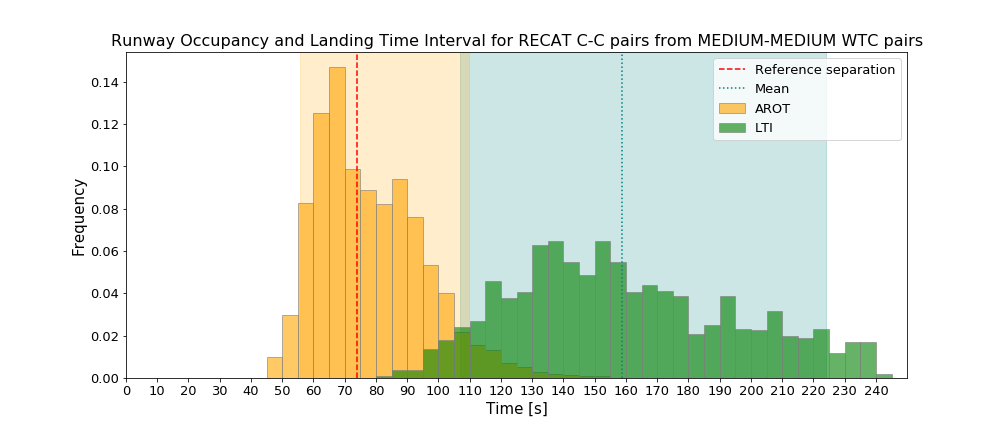
\includegraphics[width=1\textwidth]{graphics/fig_CC_from_MM_pairs_time_sep.png}
    \caption[AROT and LTI of C-C pairs originating from ICAO M-M pairs]{AROT and landing time intervals of C-C pairs originating from ICAO M-M pairs. The dashed red line indicates the RECAT-EU reference time separation for the C-C pairs. The blue horizontal line indicates 2 standard deviation left and right of the mean.}
    \label{fig:CC_from_MM_pairs_time_sep}
\end{figure}

Nevertheless the potential for decrease of the landing time interval was hindered by the AROT, the other major factor affecting runway capacity (refer to \ref{sec:runway_capacity}). All of the distributions in the figures above witness an overlap of the reference time separation line and the AROT frequency distribution. The average runway occupancy time was estimated as 77,5 seconds (\ref{ssec:runway_usage_arot}) and compared to the reference time line for the predominant C-C pairs (74 seconds), it is apparent that the AROT is the limiting factor and a major constraint for shift in the LTI distribution.








% \lipsum[28-34]

%%% Local Variables: 
%%% mode: latex
%%% TeX-master: "DEGREE-NAME-YEAR"
%%% End: 
